\chapter{Results}
% \textit{\ifdraft{In this section you discuss any issues that came up while developing
% the system. If you found something particularly interesting,
% difficult, or an important learning experience, put it here. This is
% also a good place to put additional figures and data.}}
The experimental results and evaluation of the proposed concept are covered in this chapter. Section \ref{resrobotcontrol} shows how the robot performed moving objects and creating new arrangements. Section \ref{rescamera} shows results from the automatically labelling. Section \ref{sec:resneural} shows results from the neural networks on images with objects in a bin. 

\section{Using a robot to create image data set}\label{resrobotcontrol}
%\textbf{Robot manipulator performance was measured by making tests on two products and measuring time, iterations, and interventions needed.} 
The performance of the Robot manipulator can be seen in \textit{Table \ref{tab:testonrobot}}, it has the item name, start position of the item in world-coordinates, how often the robot moved the object, how often the operator needed to interfere with the robot and help the robot to pick the object, time in seconds, whether the robot finished all the iterations without failing, how long it takes the robot to move one object and how often it needed intervention versus iterations. 


\vspace{1cm}
\begin{table}[h]
\resizebox{\textwidth}{!}{%
\begin{tabular}{clccccccc}
\hline
\textit{Test\#} &
 \textit{Item} &
 \textit{\begin{tabular}[c]{@{}c@{}}Start pos\\ {[}x, y, z{]}\end{tabular}} &
 \textit{Iterations} &
 \textit{\begin{tabular}[c]{@{}c@{}}Operator\\ intervention\end{tabular}} &
 \textit{\begin{tabular}[c]{@{}c@{}}Time \\ {[}sec{]}\end{tabular}} &
 \textit{\begin{tabular}[c]{@{}c@{}}Did it \\ finish?\end{tabular}} &
 \textit{\begin{tabular}[c]{@{}c@{}}Movement \\ time {[}sec{]}\end{tabular}} &
 \textit{\begin{tabular}[c]{@{}c@{}}Intervention\\ vs. Iterations\end{tabular}} \\ \hline
\multicolumn{1}{c|}{1} &
 \begin{tabular}[c]{@{}l@{}}Nivea \\ Cleansing Milk\end{tabular} &
 \begin{tabular}[c]{@{}c@{}}{[}0.336, \\ 0.045, \\ 0.097{]}\end{tabular} &
 100 &
 2 &
 1277.2 &
 Yes &
 12.77 &
 2.00\% \\
\multicolumn{1}{c|}{2} &
 \begin{tabular}[c]{@{}l@{}}Alberto \\ Balsam coconut\end{tabular} &
 \begin{tabular}[c]{@{}c@{}}{[}0.343, \\ 0.043, \\ 0.107{]}\end{tabular} &
 100 &
 0 &
 1254.2 &
 Yes &
 12.54 &
 0.00\% \\
\multicolumn{1}{c|}{3} &
 \begin{tabular}[c]{@{}l@{}}Nivea \\ Cleansing Milk\end{tabular} &
 \begin{tabular}[c]{@{}c@{}}{[}0.340 , \\ 0.044, \\ 0.098{]}\end{tabular} &
 300 &
 6 &
 3799.1 &
 Yes &
 12.66 &
 2.00\% \\
\multicolumn{1}{c|}{4} &
 \begin{tabular}[c]{@{}l@{}}Alberto \\ Balsam coconut\end{tabular} &
 \begin{tabular}[c]{@{}c@{}}{[}0.333 , \\ -0.040, \\ 0.118{]}\end{tabular} &
 300 &
 1 &
 3774.4&
 Yes &
 12.58 &
 0.33\% \\ \hline
\multicolumn{7}{r}{\textbf{Average:}} &
 12.64 &
 1.08\% \\ 
\end{tabular}%
}
\caption{Test made on the robot and code performance}
\label{tab:testonrobot}
\end{table}
The most common intervention situations are when the robot would not pick the object or some part of the robot end-effector crashed into the bin, since that happened the end effector was extended by 14 cm. The new extended end effector can be seen in the method chapter in \textit{Figure \ref{figure: newendeffector}}. When the robot end effector had been extended the robot worked every time without any operator intervention.
\clearpage
%%%%%%%%%%%%%%%%%%%%%%%%%%%%%%%%%%%%%%%%%%%%%%%%%%%%%%%%%%%%%%%%%%%%%
\section{Automatic labelling}\label{rescamera}
This section shows results from the automatically labelling for two different methods.

\subsection{Before vs. after}\label{subsec:beforeafter}
\begin{figure}[ht]
 \centering
 % include first image
 \subfloat[Before]{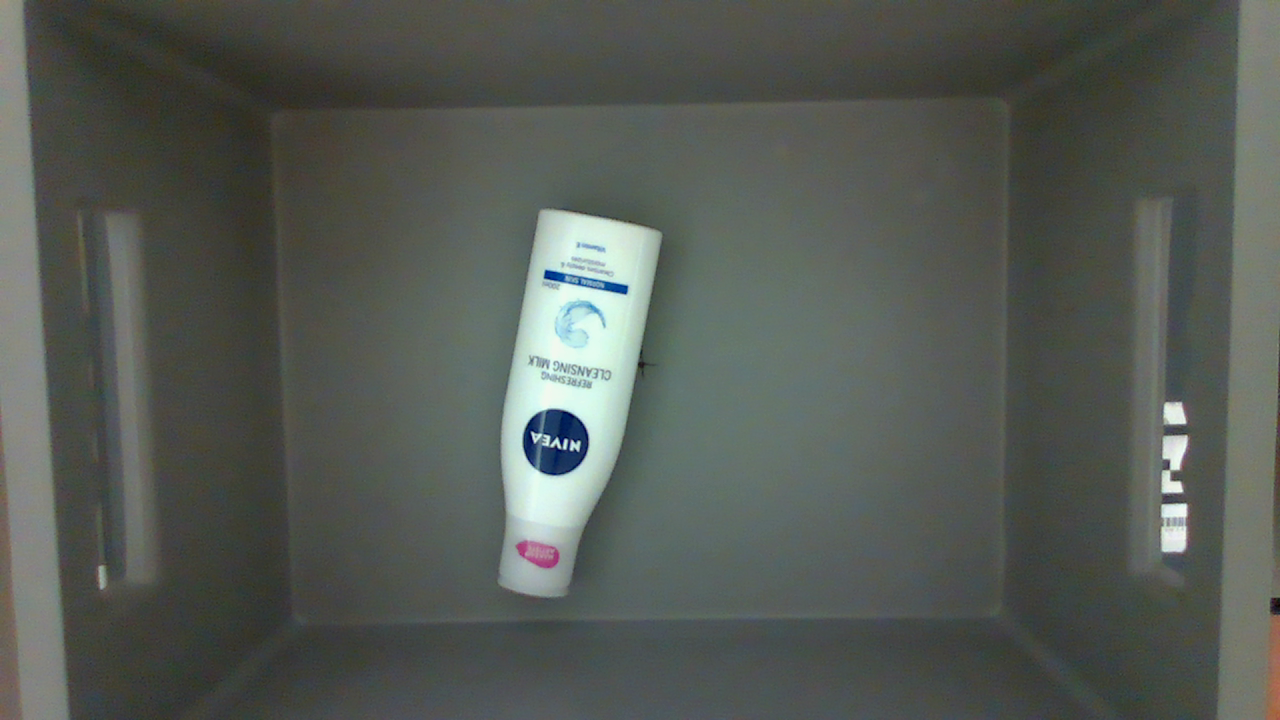
\includegraphics[width=0.35\textwidth]{graphics/results/tbefore.png}}
 \hspace{0.5cm}
 \subfloat[After]{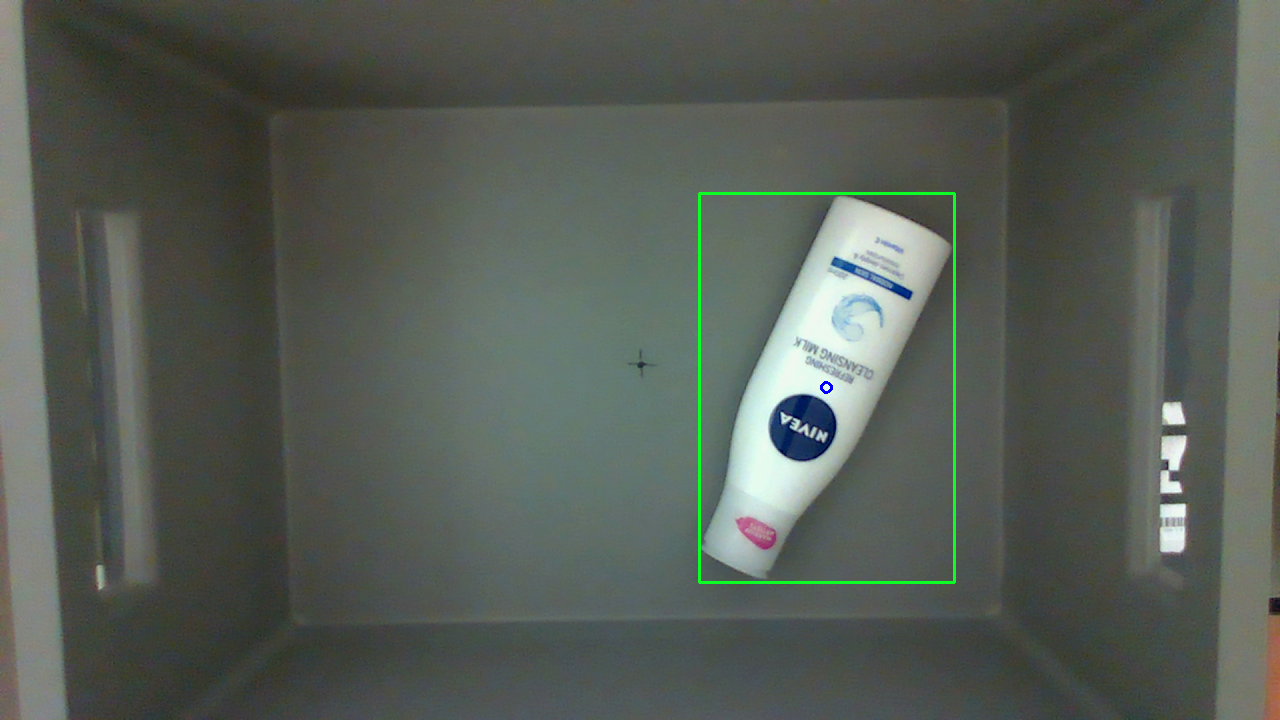
\includegraphics[width=0.35\textwidth]{graphics/results/tafter.png}}
 \hspace{0.5cm}
 \subfloat[Contours]{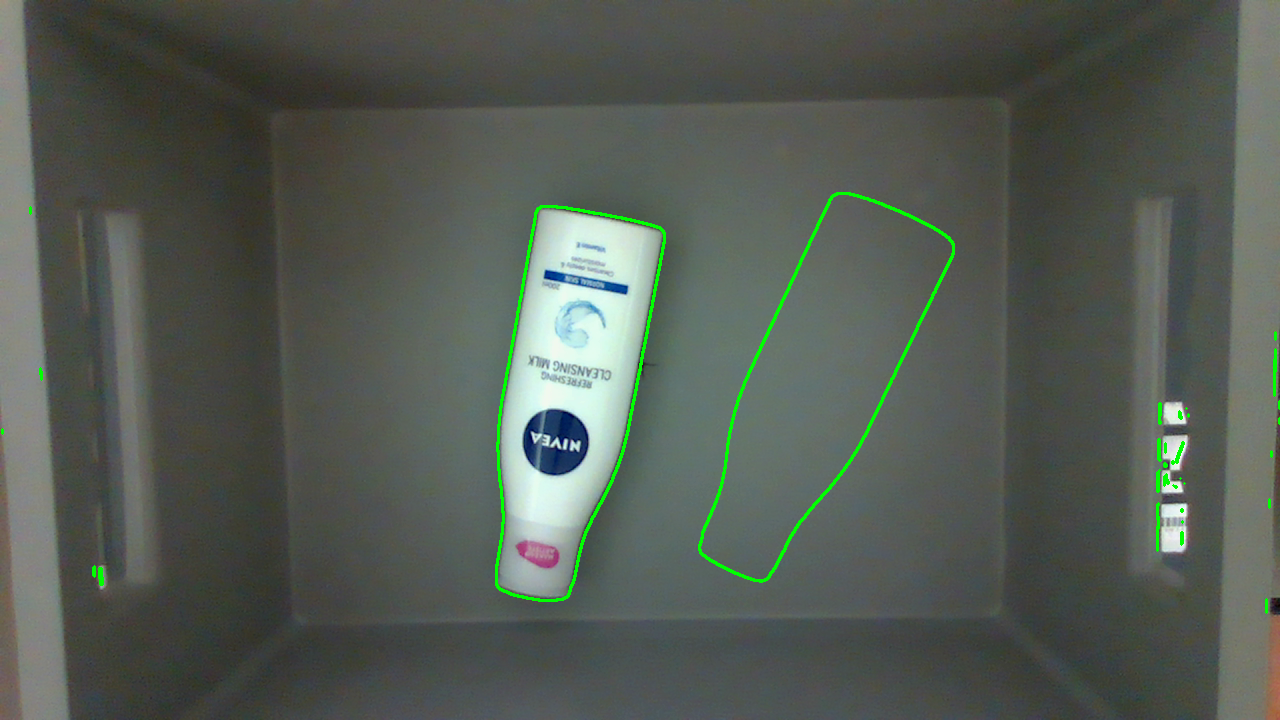
\includegraphics[width=0.35\textwidth]{graphics/results/tmask1.png}}
 \hspace{0.5cm}
 \subfloat[Masked]{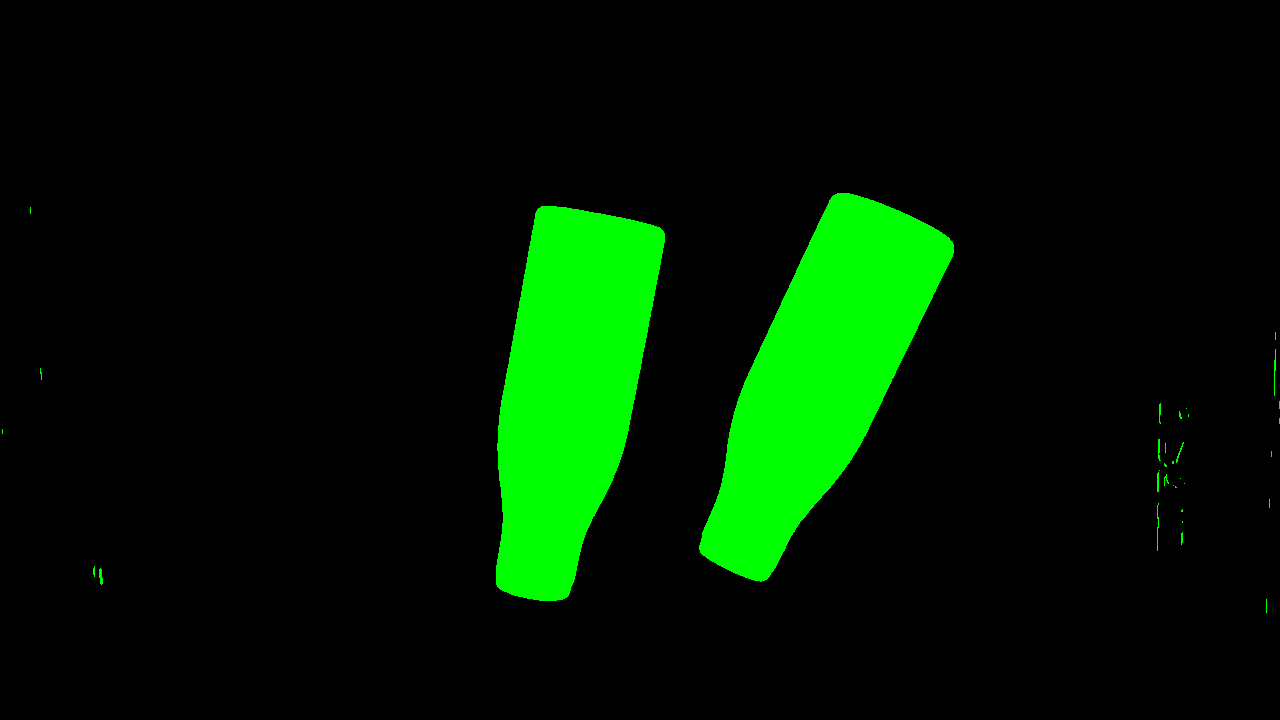
\includegraphics[width=0.35\textwidth]{graphics/results/tmasked.png}}
 \caption{Image Difference with OpenCV and Python, example of good annotation}
 \label{figure: imagework1}
\end{figure}

\begin{figure}[ht]
 \centering
 % include first image
 \subfloat[Before]{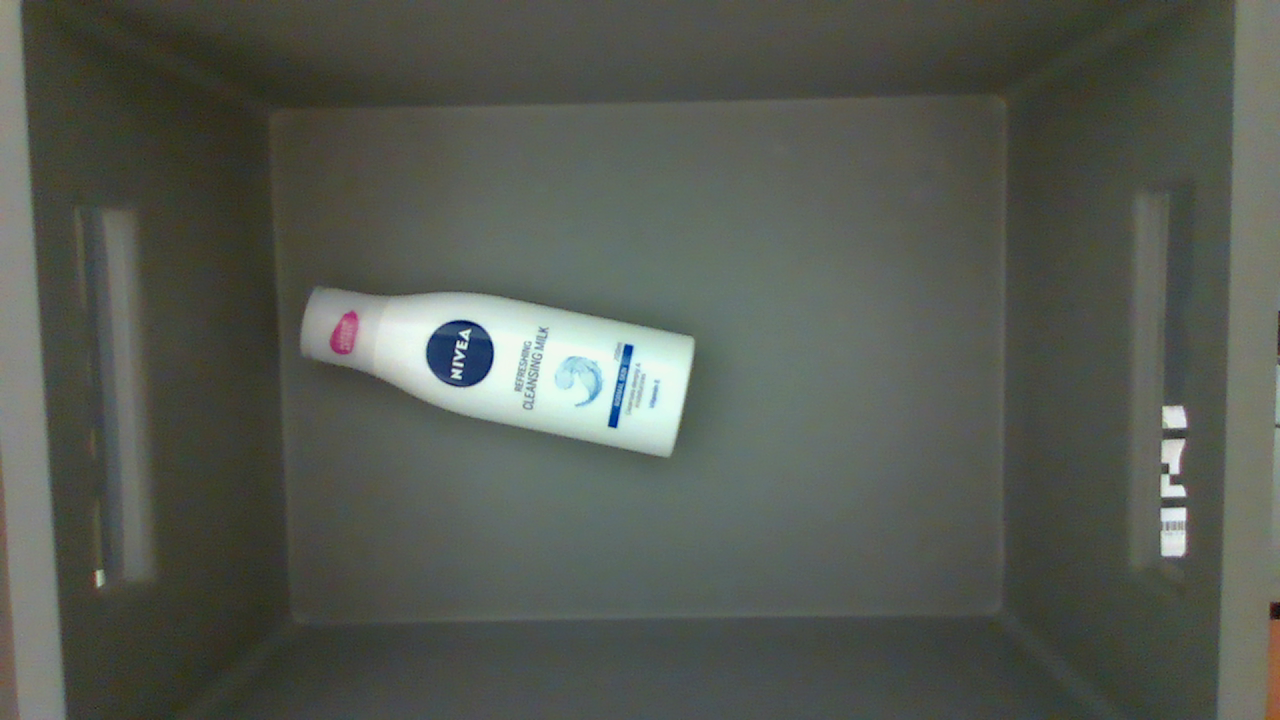
\includegraphics[width=0.35\textwidth]{graphics/9before.png}}
 \hspace{0.5cm}
 \subfloat[After]{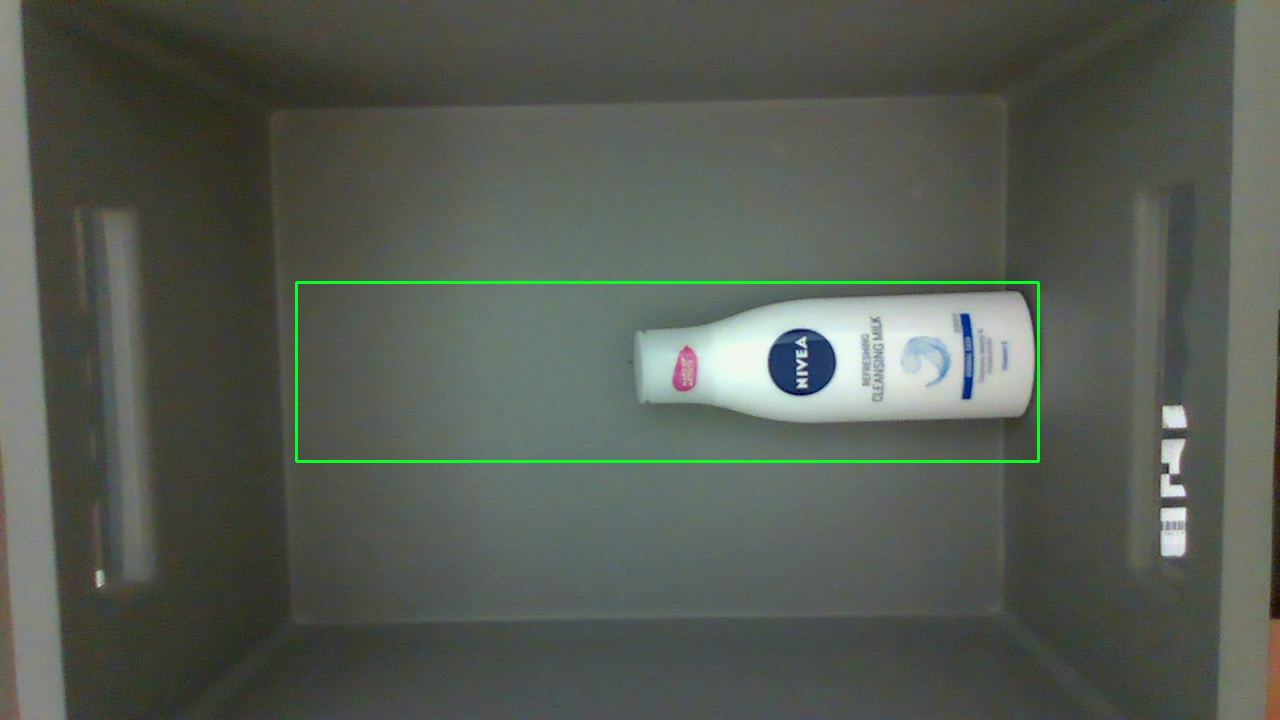
\includegraphics[width=0.35\textwidth]{graphics/9after.png}}
 \hspace{0.5cm}
 \subfloat[Contours]{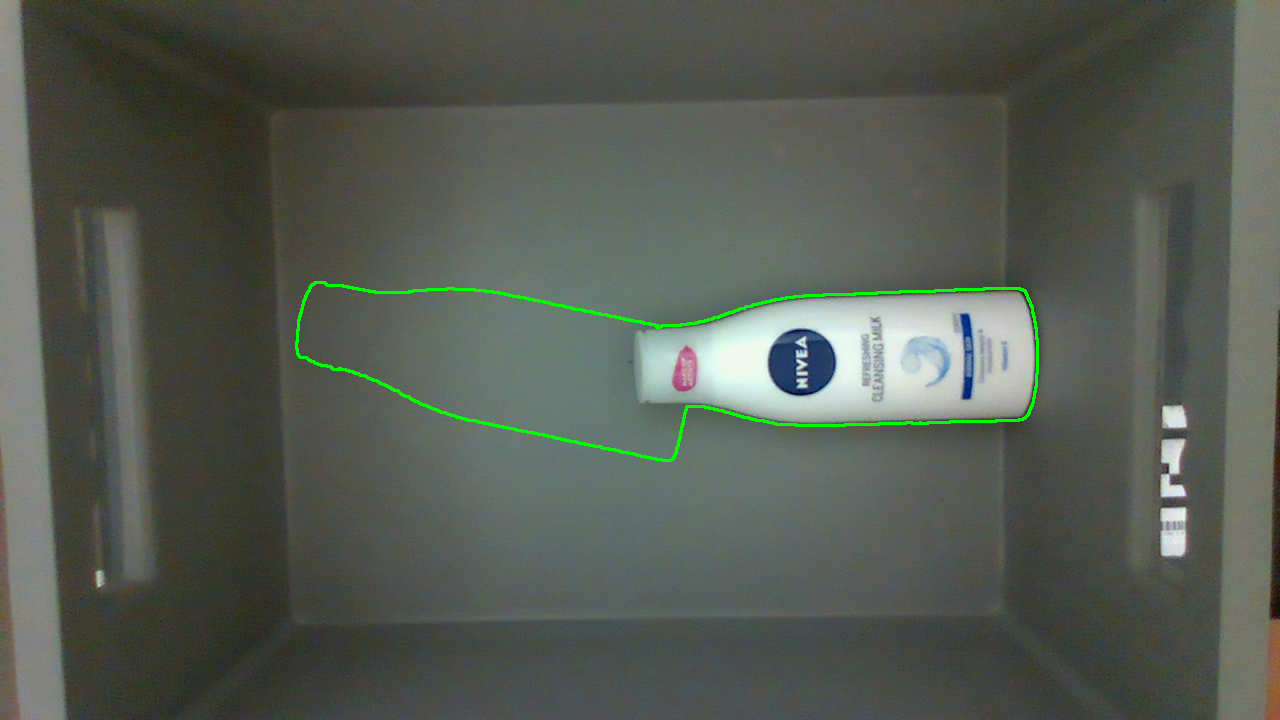
\includegraphics[width=0.35\textwidth]{graphics/9filled.png}}
 \hspace{0.5cm}
 \subfloat[Masked]{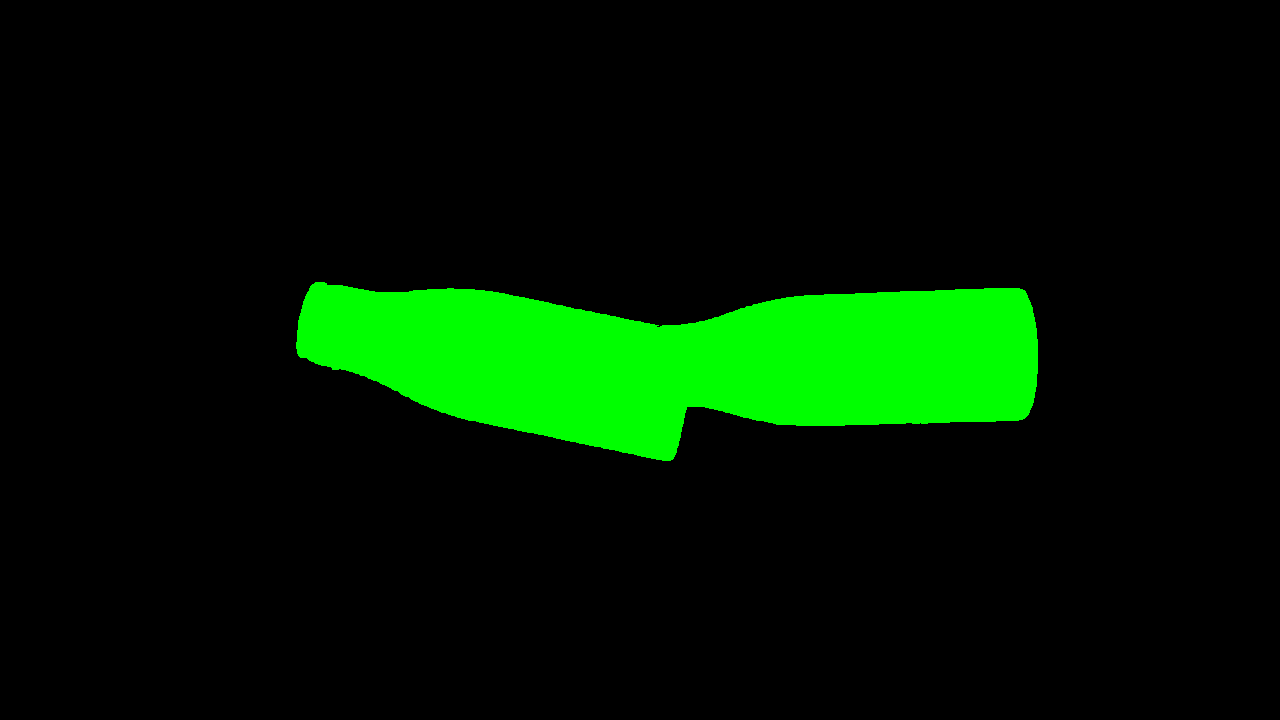
\includegraphics[width=0.35\textwidth]{graphics/9masked.png}}
 \caption{Image Difference with OpenCV and Python, example of bad annotation}
 \label{figure: imagework2}
\end{figure}

In \textit{Figure \ref{figure: imagework1}} and \textit{Figure \ref{figure: imagework2}} shows an example of good and bad automatic annotation. The figures show the item in before position and after position with only one object in the bin. In the bottom row the contoured difference and masked contour area can be seen. 
\clearpage
\begin{figure}[ht]
 \centering
 % include first image
 \subfloat[Before]{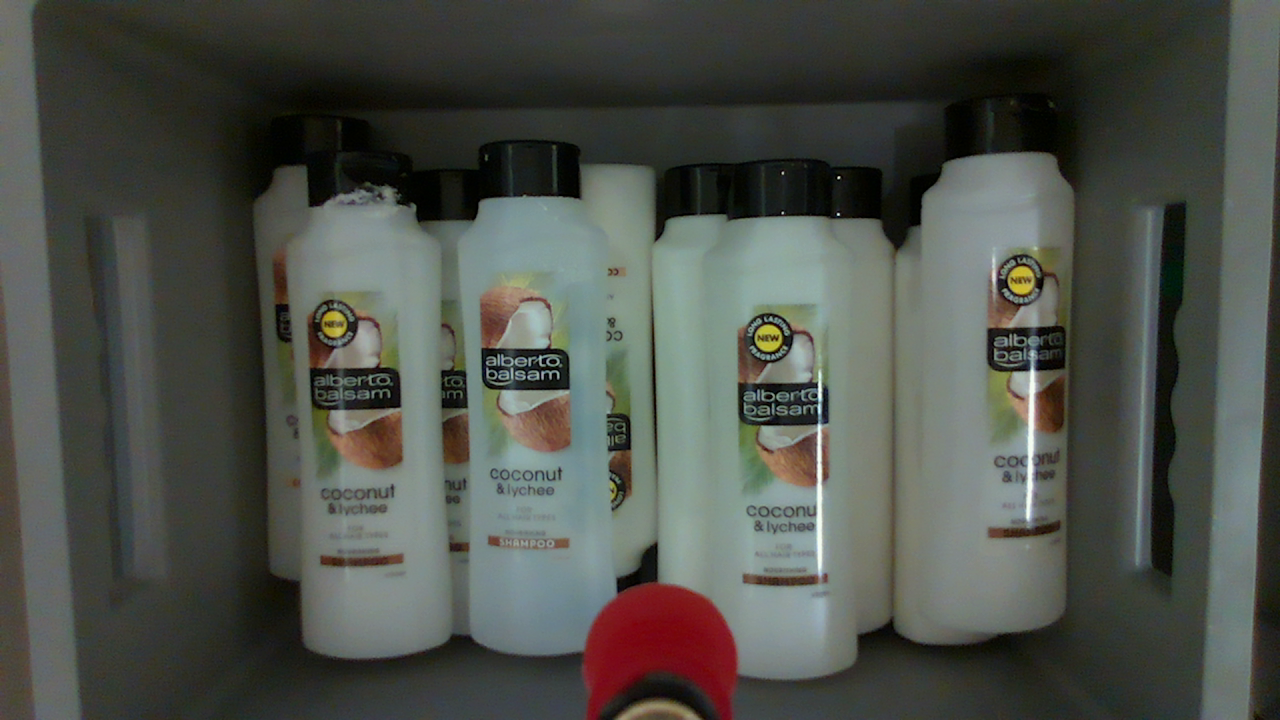
\includegraphics[width=0.4\textwidth]{graphics/results/newmulti-0019.png}}
 \hspace{0.5cm}
 \subfloat[After]{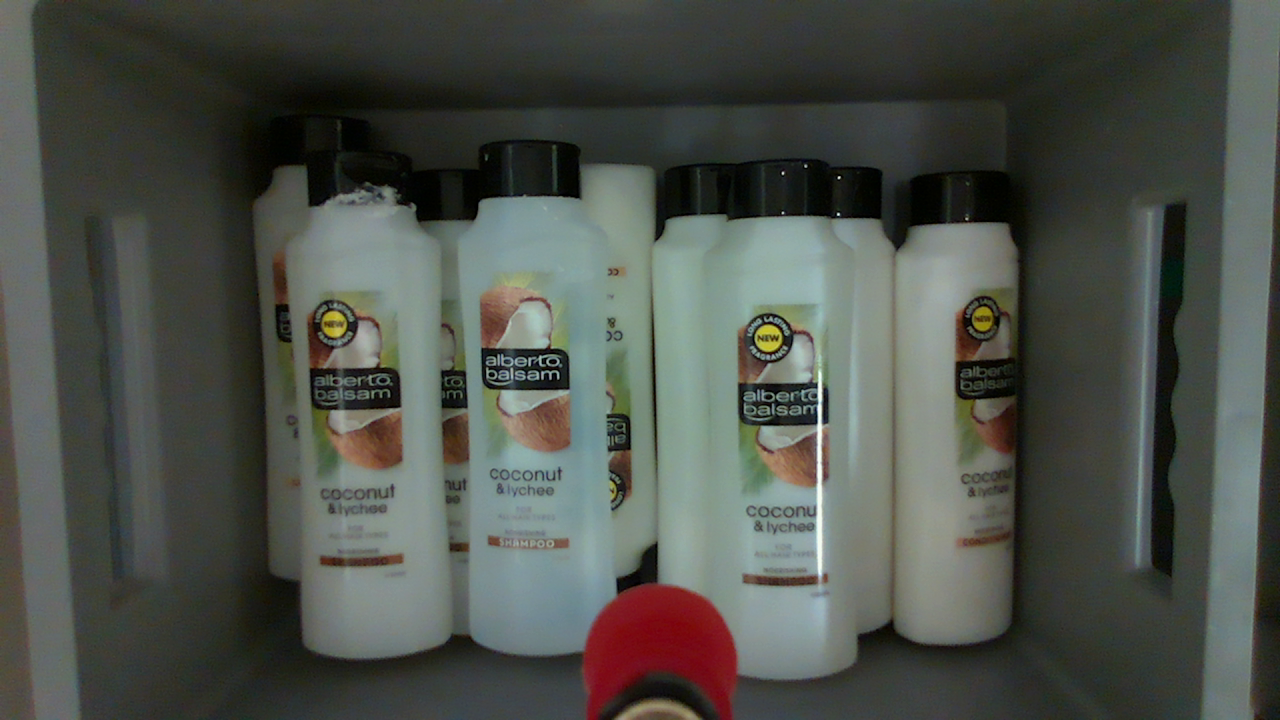
\includegraphics[width=0.4\textwidth]{graphics/results/newmulti-0020.png}}
 \hspace{0.5cm}
 \subfloat[Contours]{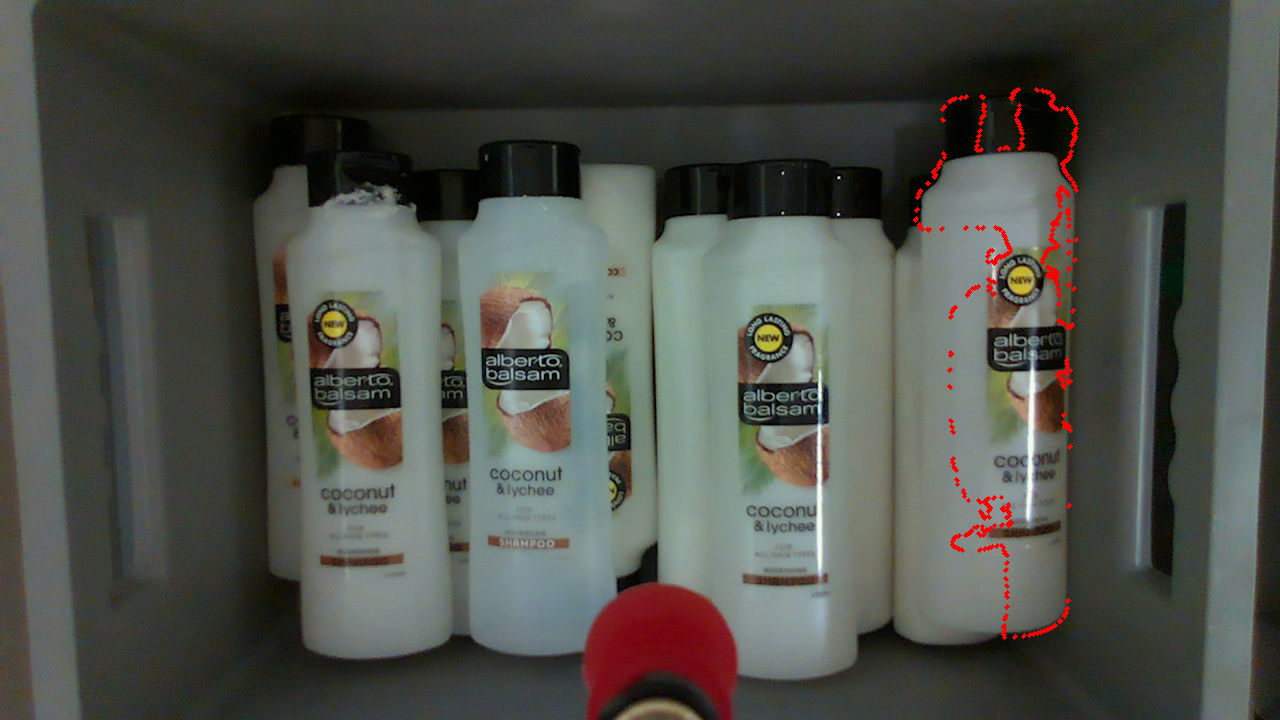
\includegraphics[width=0.4\textwidth]{graphics/results/newmulti-0019diff.png}}
 \hspace{0.5cm}
 \subfloat[Annotated]{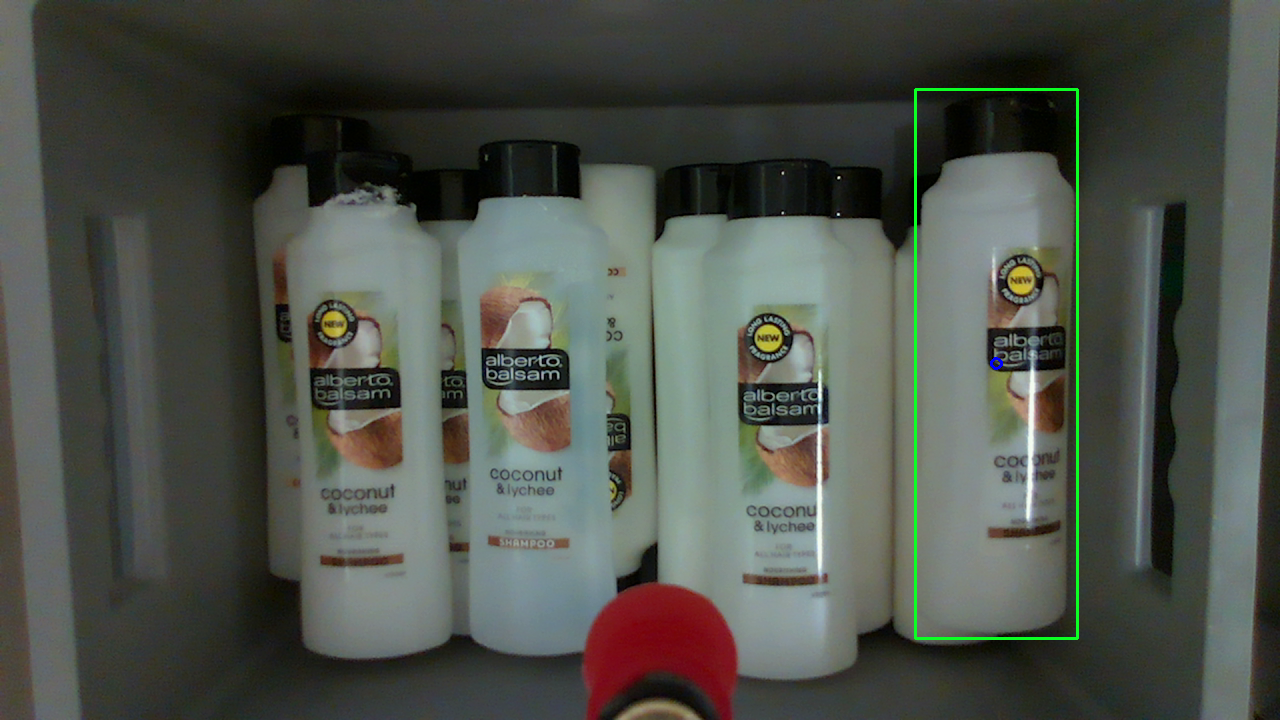
\includegraphics[width=0.4\textwidth]{graphics/results/newmulti-0019marked.png}}
 \caption{Image Difference with OpenCV and Python, example of good annotation, with multiple objects in the bin}
 \label{figure: multiimagework1}
\end{figure}

\begin{figure}[ht]
 \centering
 % include first image
 \subfloat[Before]{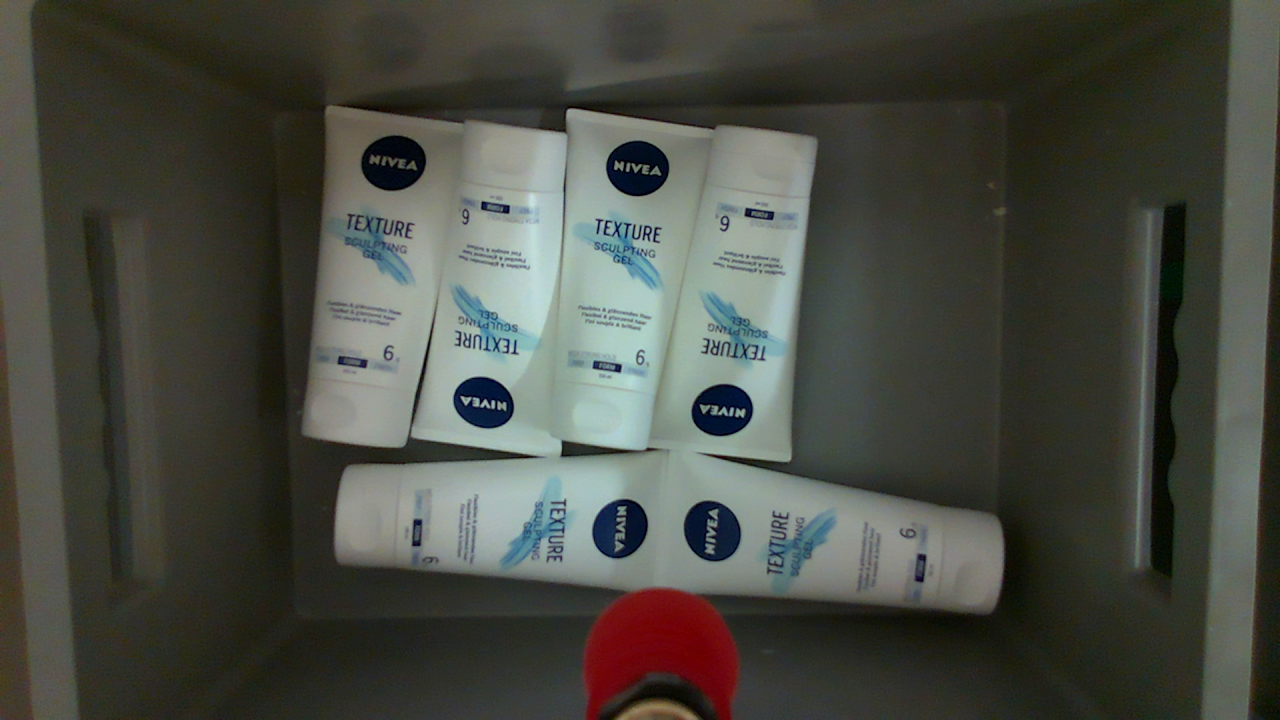
\includegraphics[width=0.4\textwidth]{graphics/results/newmulti-0051.png}}
 \hspace{0.5cm}
 \subfloat[After]{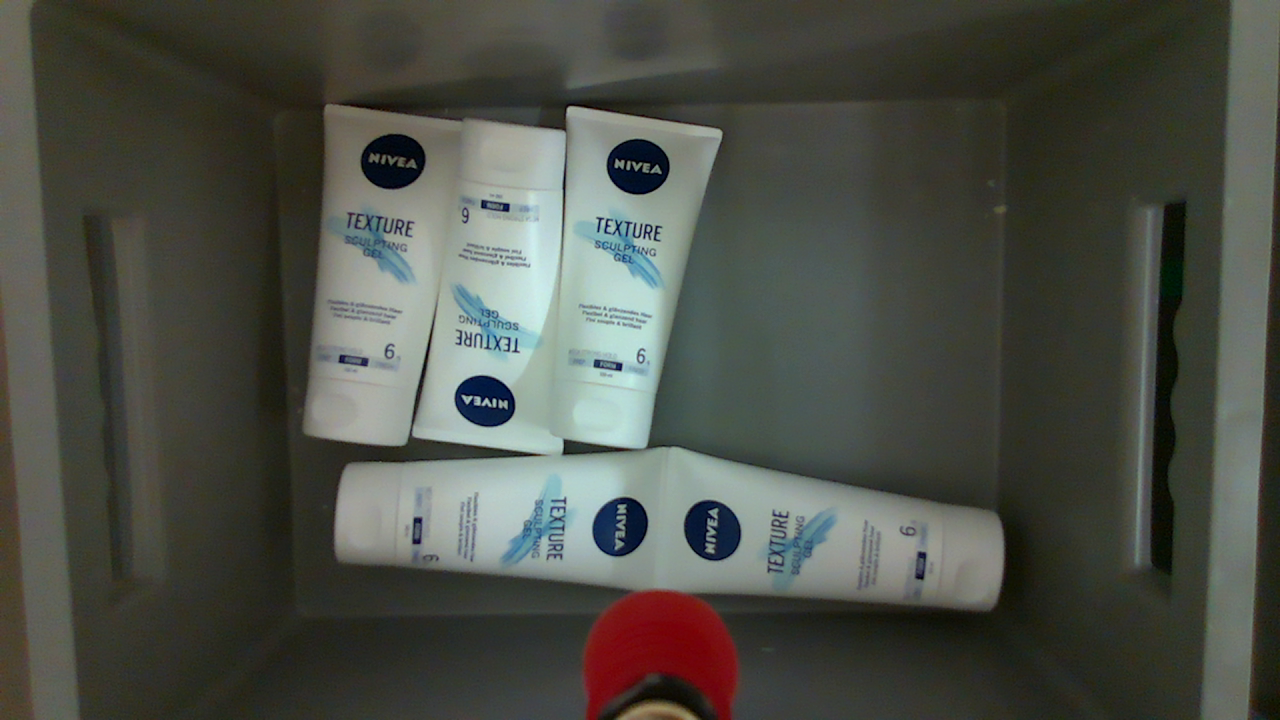
\includegraphics[width=0.4\textwidth]{graphics/results/newmulti-0052.png}}
 \hspace{0.5cm}
 \subfloat[Contours]{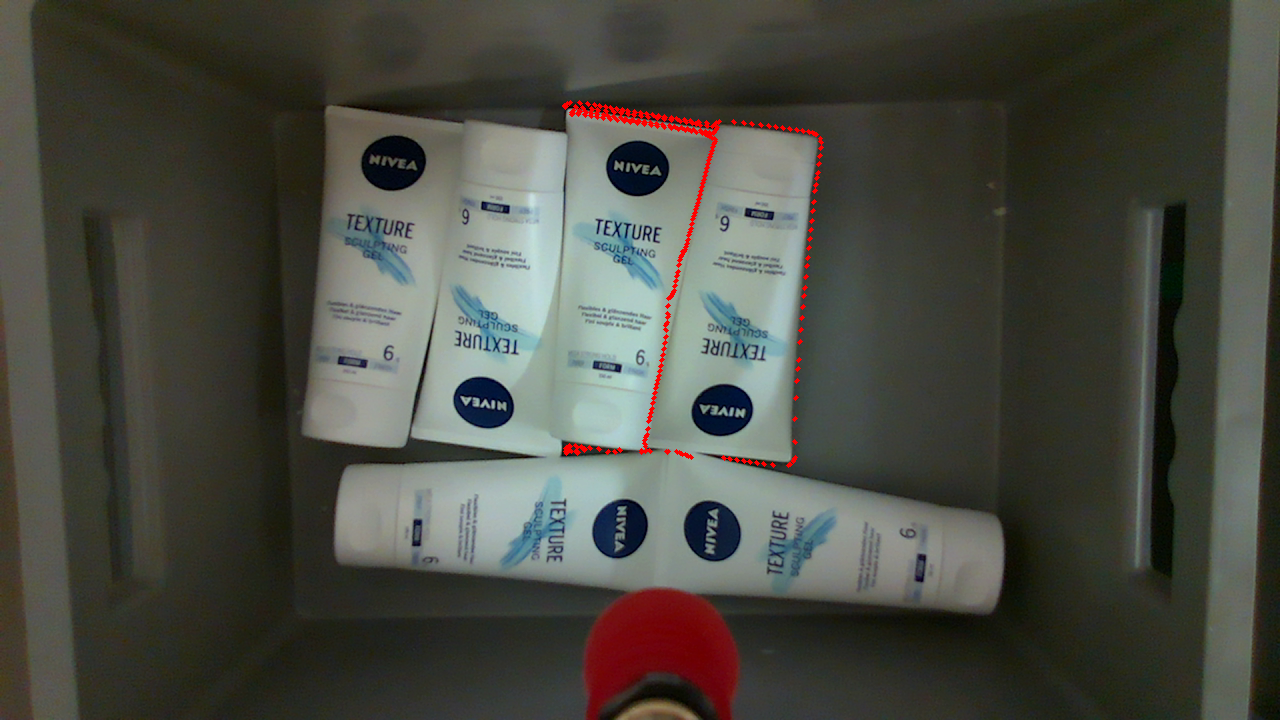
\includegraphics[width=0.4\textwidth]{graphics/results/newmulti-0051diff.png}}
 \hspace{0.5cm}
 \subfloat[Annotated]{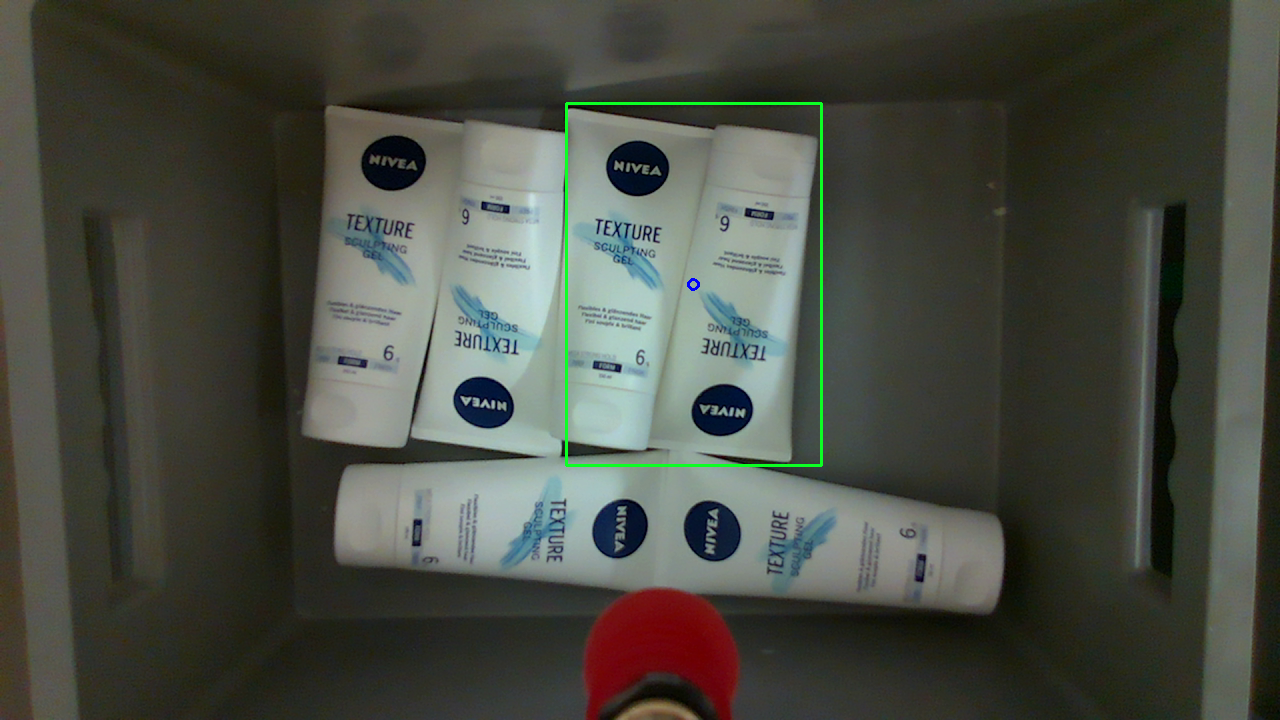
\includegraphics[width=0.4\textwidth]{graphics/results/newmulti-0051marked.png}}
 \caption{Image Difference with OpenCV and Python, example of bad annotation, with multiple objects in the bin}
 \label{figure: multiimagework2}
\end{figure}

In \textit{Figure \ref{figure: multiimagework1}} and \textit{Figure \ref{figure: multiimagework2}} shows an example of good and bad automatic annotation. The figures show an example of a before and after image when removing one object when there are multiple items in the bin. In the bottom row, the contoured difference and annotated object area can be seen. %The reason for bad annotation is because the two objects moved and not only one. 

\clearpage
\subsection{Empty bin vs. Object in the bin} \label{subsec:emptybin}
\begin{figure}[h]
 \centering
 % include first image
 \subfloat[Before annotation]{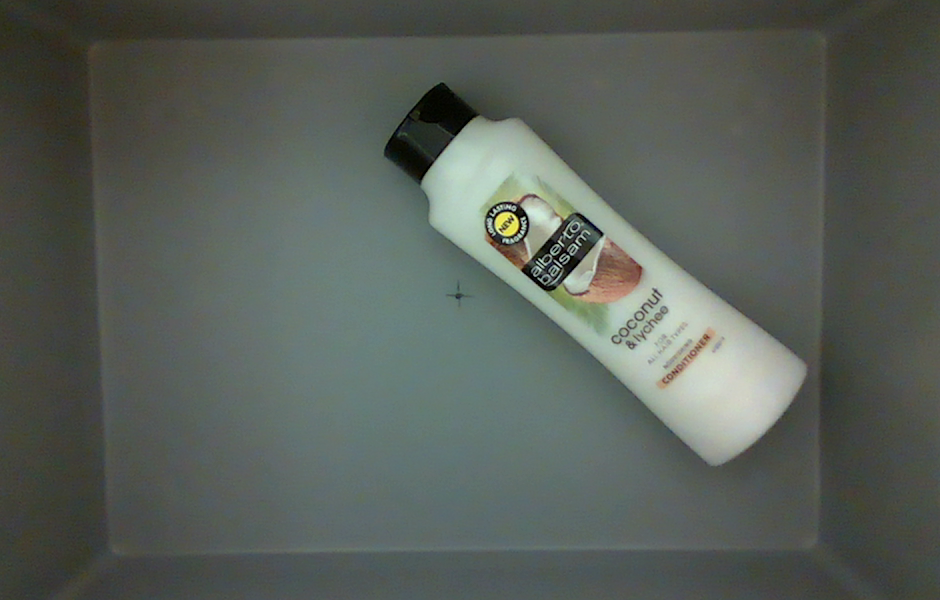
\includegraphics[width=0.4\textwidth]{graphics/results/9img3.png}}
 \hspace{0.5cm}
 \subfloat[Contours]{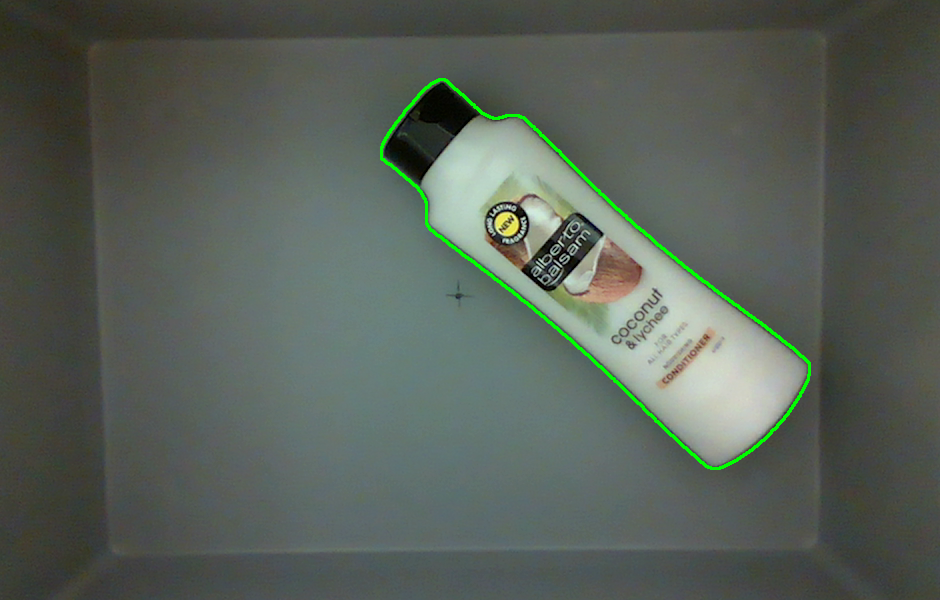
\includegraphics[width=0.4\textwidth]{graphics/results/9diff.png}}
 \hspace{0.5cm}
 \subfloat[Masked]{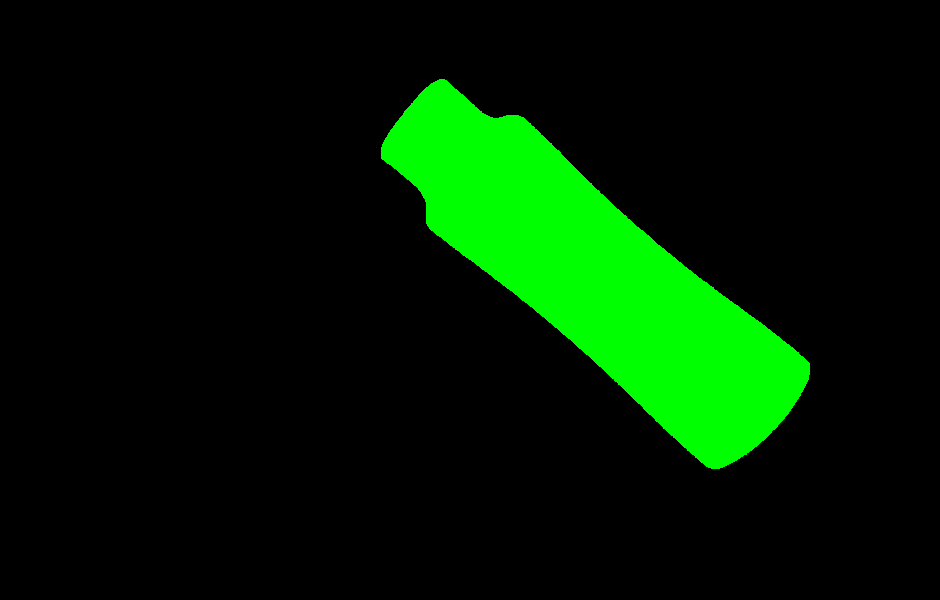
\includegraphics[width=0.4\textwidth]{graphics/results/9img1.png}}
 \hspace{0.5cm}
 \subfloat[After annotation]{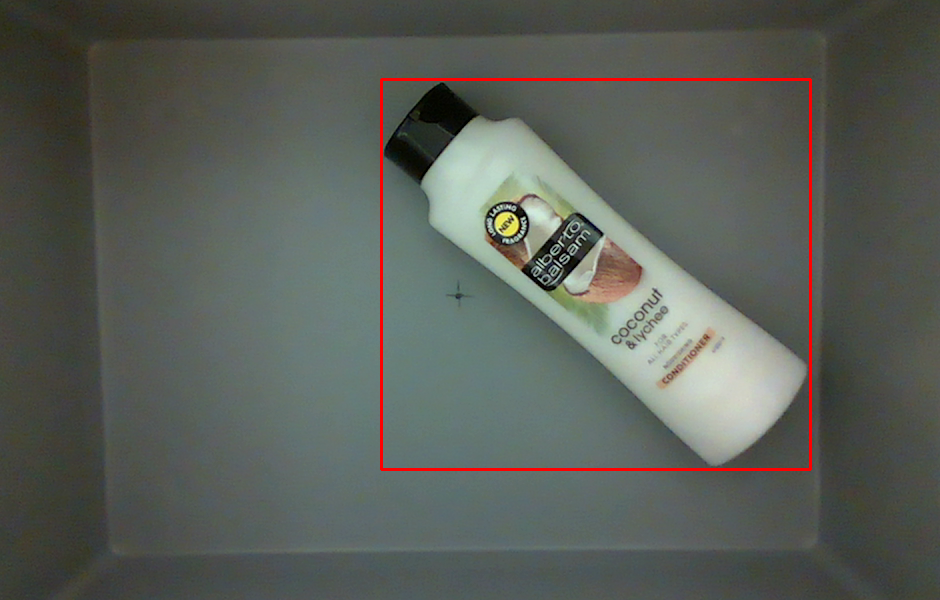
\includegraphics[width=0.4\textwidth]{graphics/results/9img2.png}}
 \caption{An example of good annotation, from the empty bin vs. one item in the bin method}
 \label{figure: labelling}
\end{figure}

\begin{figure}[h]
 \centering
 % include first image
 \subfloat
 [Before annotation]{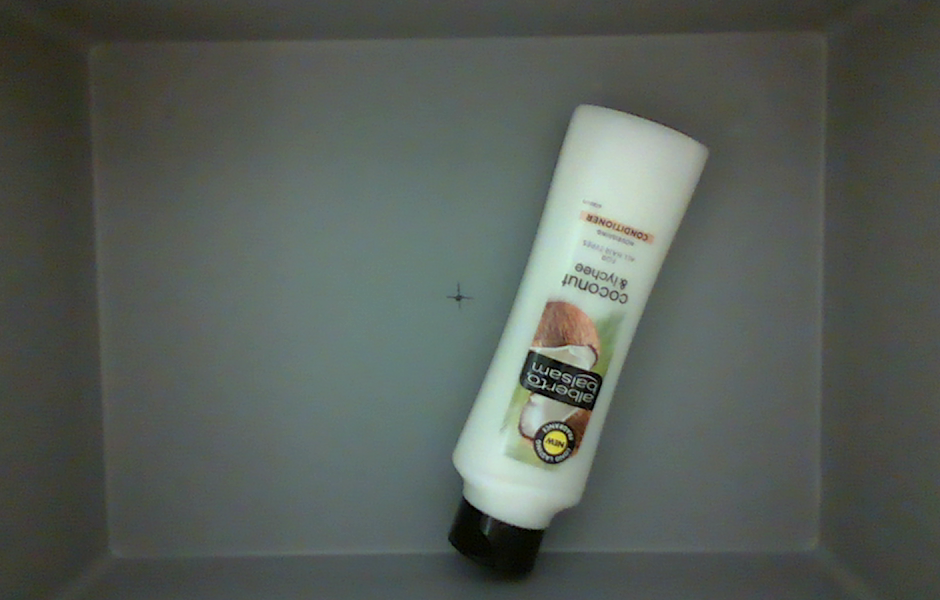
\includegraphics[width=0.4\textwidth]{graphics/results/48img3.png}}
 \hspace{0.5cm}
 \subfloat[Contours]{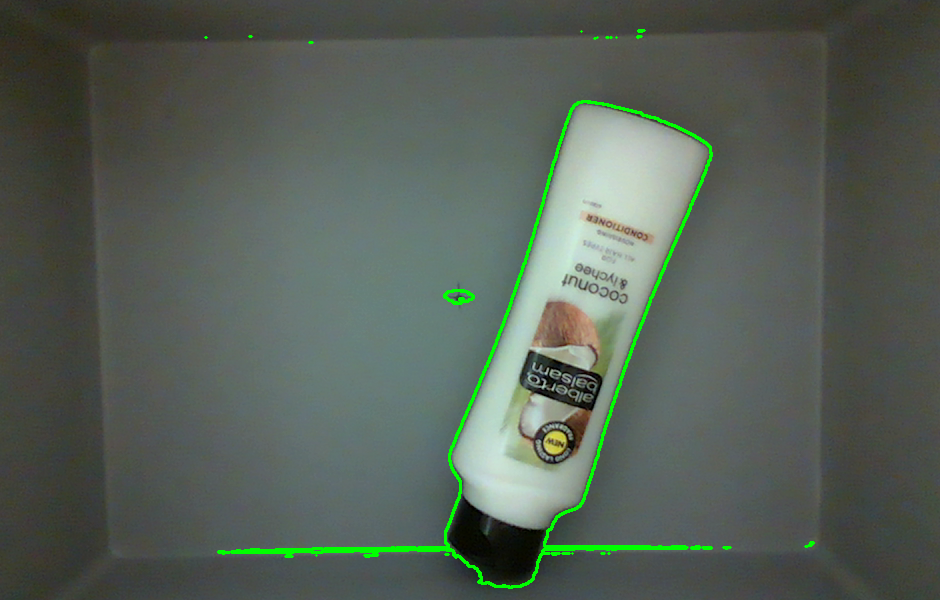
\includegraphics[width=0.4\textwidth]{graphics/results/48diff.png}}
 \hspace{0.5cm}
 \subfloat[Masked]{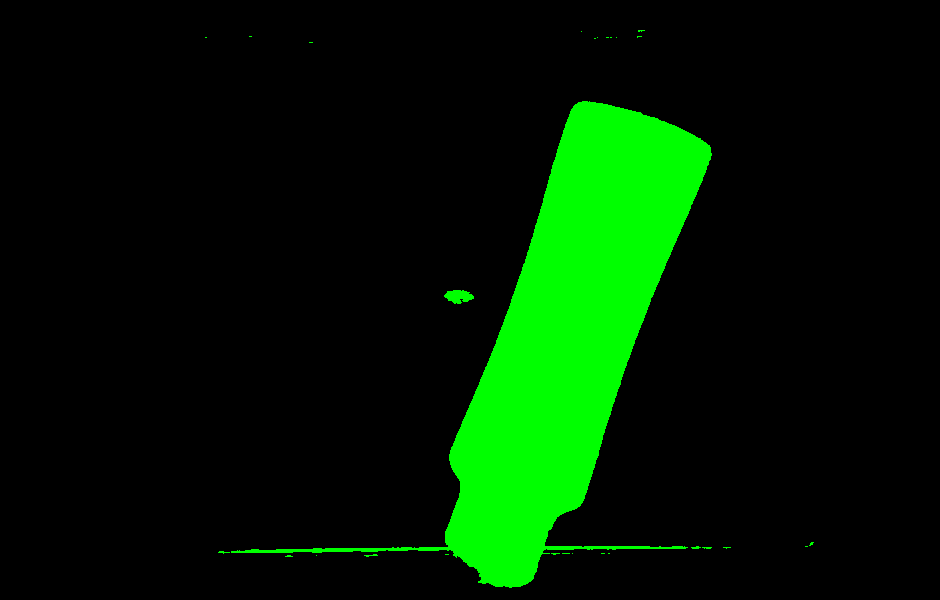
\includegraphics[width=0.4\textwidth]{graphics/results/48img1.png}}
 \hspace{0.5cm}
 \subfloat[After annotation]{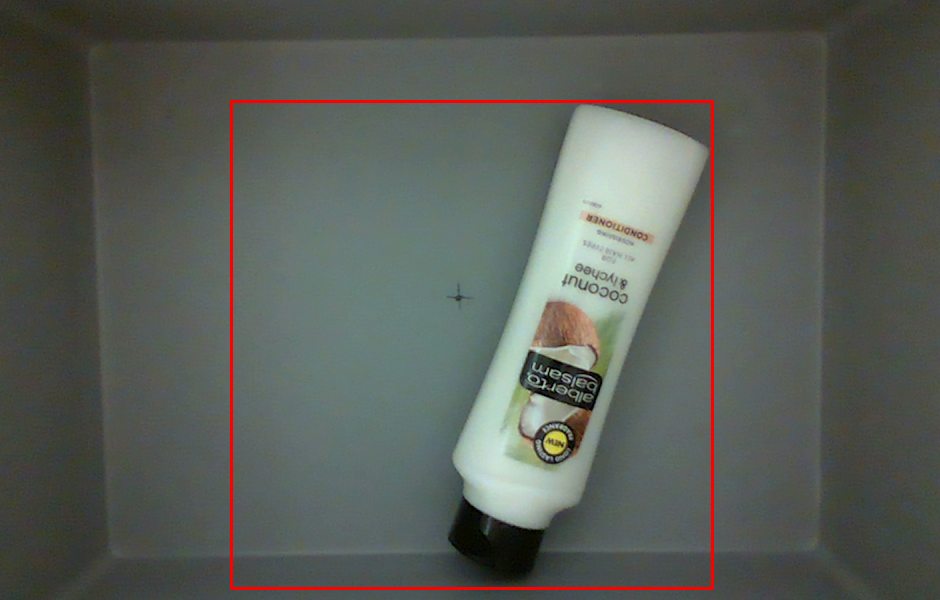
\includegraphics[width=0.4\textwidth]{graphics/results/48img2.png}}
 \caption{An example of bad annotation, from the empty bin vs. one item in the bin method}
 \label{figure: badlabelling}
\end{figure}
%As can been seen in the \textit{Figure \ref{figure: labelling}} this method can be used to find the bounding box and to create a automatic labelled data. 
\textit{Figure \ref{figure: labelling}} and \textit{Figure \ref{figure: badlabelling}} shows examples of successful and failed boundary box annotation, as determined by visual inspection. 

\clearpage

% Results from that test can been seen in \textit{Table \ref{tab:timediff}} and also it takes on average 0.85 second to label one image.

% Consider saying Figure 3.2 shows examples of successful and failed boundary box detection, as determined by visual inspection. A single example does not warrant stating that a method can be used. Leave this to the discussion, where you take into account the results of the visual inspection. Consider adding more examples and a table with the number of successful and failed boundary box detections.



\begin{table}[h]
\resizebox{\textwidth}{!}{%
\begin{tabular}{clccc}
\hline
\multicolumn{1}{l|}{\textit{Test \#}} &
 \textit{Item} &
 \multicolumn{1}{l}{\textit{Images}} &
 \multicolumn{1}{l}{\textit{Total time {[}s{]}}} &
 \multicolumn{1}{l}{\textit{Time per image {[}s{]}}} \\ \hline
\multicolumn{1}{c|}{1} & \begin{tabular}[c]{@{}l@{}}Nivea\\ cleansing milk\end{tabular} & 300 & 255.99 & 0.85 \\
\multicolumn{1}{c|}{2} & \begin{tabular}[c]{@{}l@{}}Nivea\\ cleansing milk\end{tabular} & 102 & 92.68 & 0.91 \\
\multicolumn{1}{c|}{3} & \begin{tabular}[c]{@{}l@{}}Nivea \\ elastic\end{tabular} & 72 & 56.31 & 0.78 \\
\multicolumn{1}{c|}{4} & \begin{tabular}[c]{@{}l@{}}Alberto \\ Balsam coconut\end{tabular} & 102 & 88.30 & 0.87 \\ \hline
\multicolumn{4}{r}{\textbf{Average:}} & 0.85
\end{tabular}%
}
\caption{Measured time when using the difference.py}
\label{tab:timediff}
\end{table}
A test was made on how long it would take to annotate one image. \textit{Table \ref{tab:timediff}} shows the results from that test. The average time to label one image is 0.85 seconds.

\begin{table}[h]
\resizebox{\textwidth}{!} \\ \hline
\multicolumn{1}{l|}{Alberto Balsam} & 101 & 95 & 6 & 5.9\% \\
\multicolumn{1}{l|}{Nivea Cleansing} & 102 & 102 & 0 & 0.0\% \\
\multicolumn{1}{l|}{Nivea Elastic} & 72 & 72 & 0 & 0.0\% \\
\multicolumn{1}{l|}{Nivea Texture} & 101 & 100 & 1 & 1.0\% \\ \hline
\multicolumn{4}{r}{\textbf{Average:}} & 1.9\%
\end{tabular}%
}
\caption{Annotation on the automatically generated dataset with one object in the bin }
\label{tab:annotation}
\end{table}

In \textit{Table \ref{tab:annotation}} the annotation performance is shown, it can be seen that this method returned good annotation in 98.1\% cases on average. Six automatic labelled images didn’t have good annotation and they were images 34, 50, 71, 73, 83, and 93 of the Alberto Balsam. Bad annotation is when the bounding box does not frame the object tightly and is extremely bad when the center point is unsuitable for picking.



\clearpage
%%%%%%%%%%%%%%%%%%%%%%%%%%%%%%%%%%%%%%%%%%%%%%%%%%%%%%%%%%%%%%%%%%%%%
\section{Trained neural network}\label{sec:resneural}
This section shows how the neural networks performed on images with objects in a bin.

\subsection{Results from the first neural network} \label{sec:firstneural}
\begin{figure}[h]
 \centering
 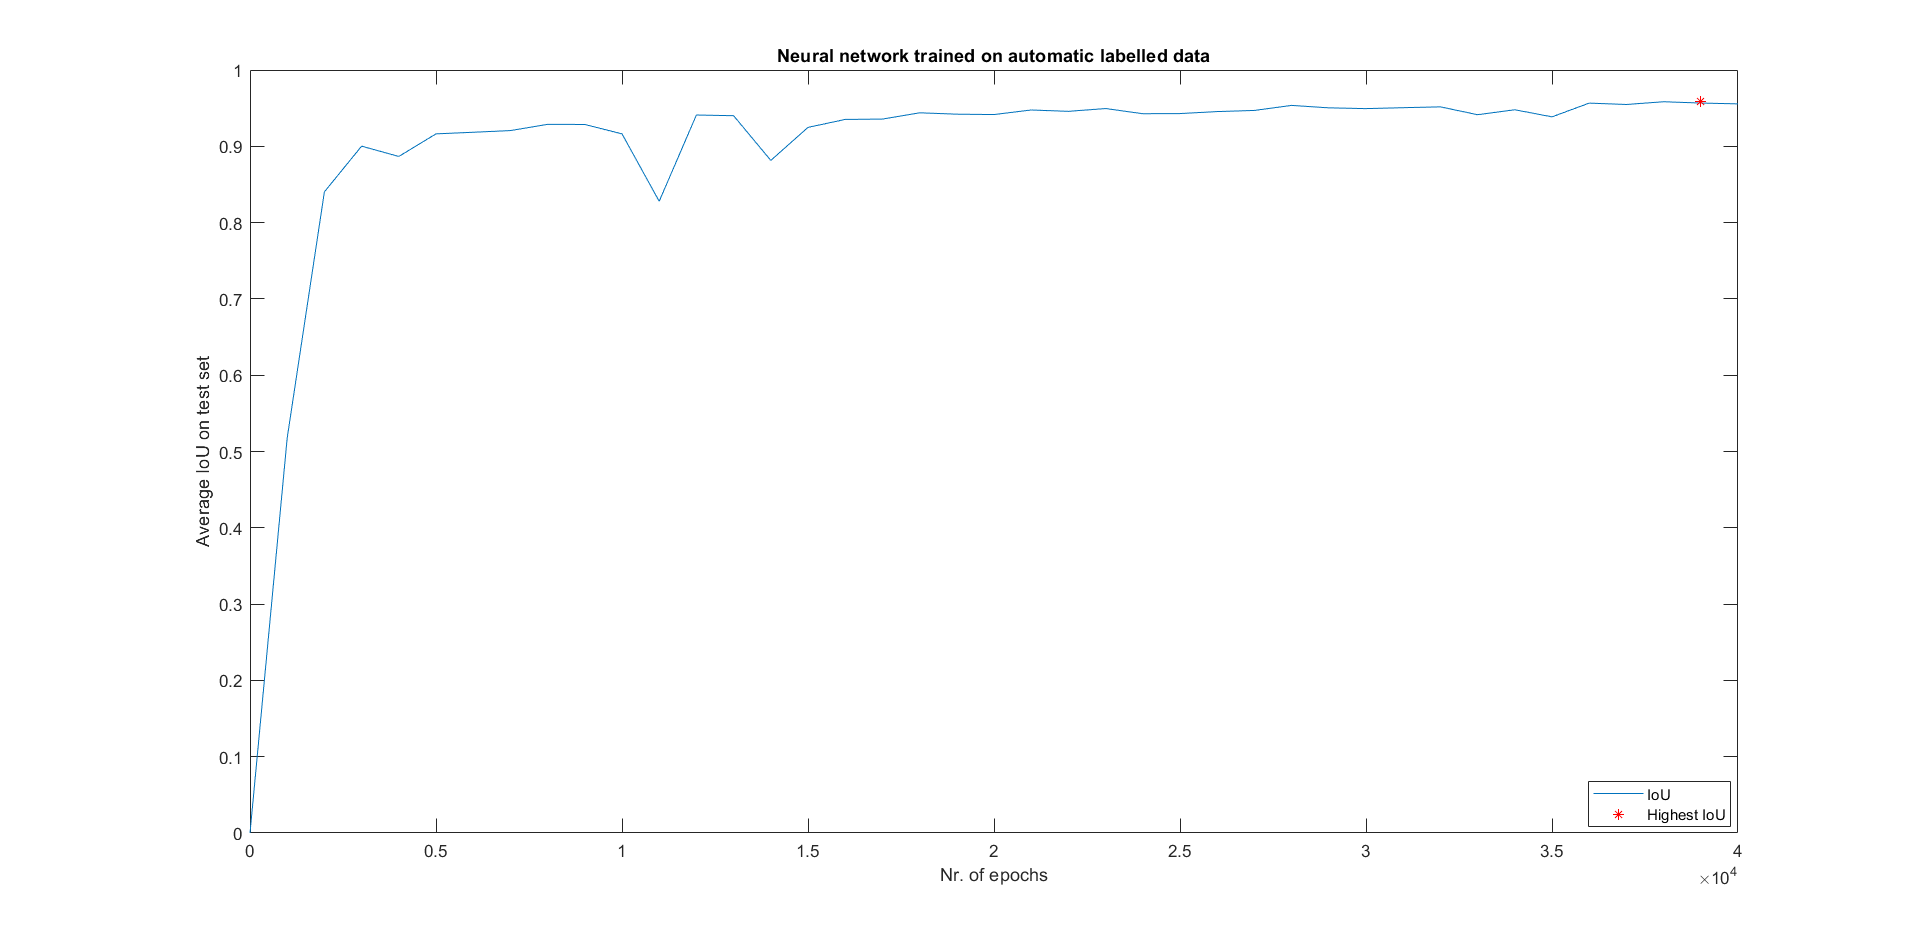
\includegraphics[width=0.8\textwidth, trim={5cm 0 4cm 0},clip]{graphics/results/neuralnetworkauto.png}
 \caption{IoU is measured over the test set on the automatically generated dataset with one object in the bin, every 1000 epochs}
 \label{fig:neuralnetwork}
\end{figure}
\textit{Figure \ref{fig:neuralnetwork}} shows how the IoU score developed over the number of epochs, when measuring over the test set. The best average IoU score can be seen in the red point and is 0.9584 at 38000 epochs. The average IoU is measured when running through the automatically generated dataset with one object in the bin(with only good annotations).

\begin{figure}[h]
 \centering
 % include first image
 \subfloat[The prior model]{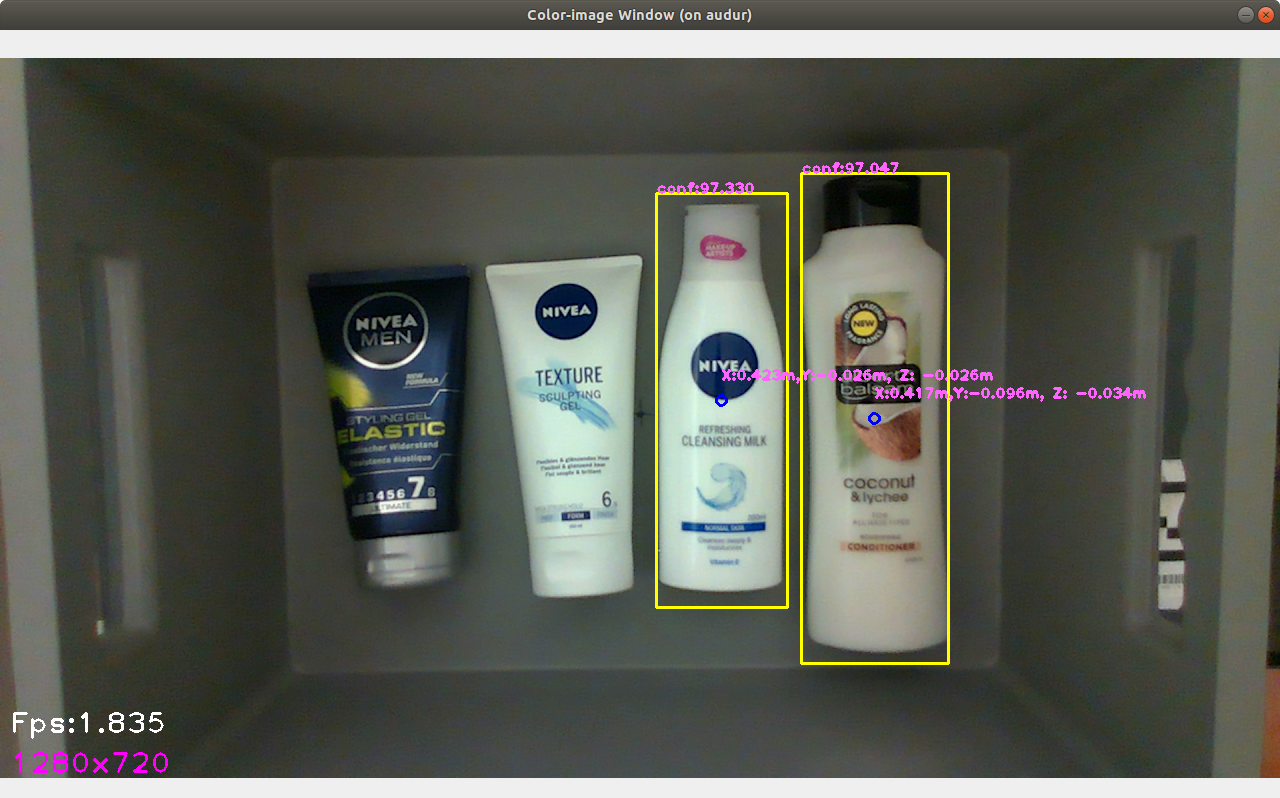
\includegraphics[width=0.3\textwidth, trim={0 0.6cm 0 2cm},clip ]{graphics/results/beforetraining.png}}
 \hfill
 \subfloat[The prior model]{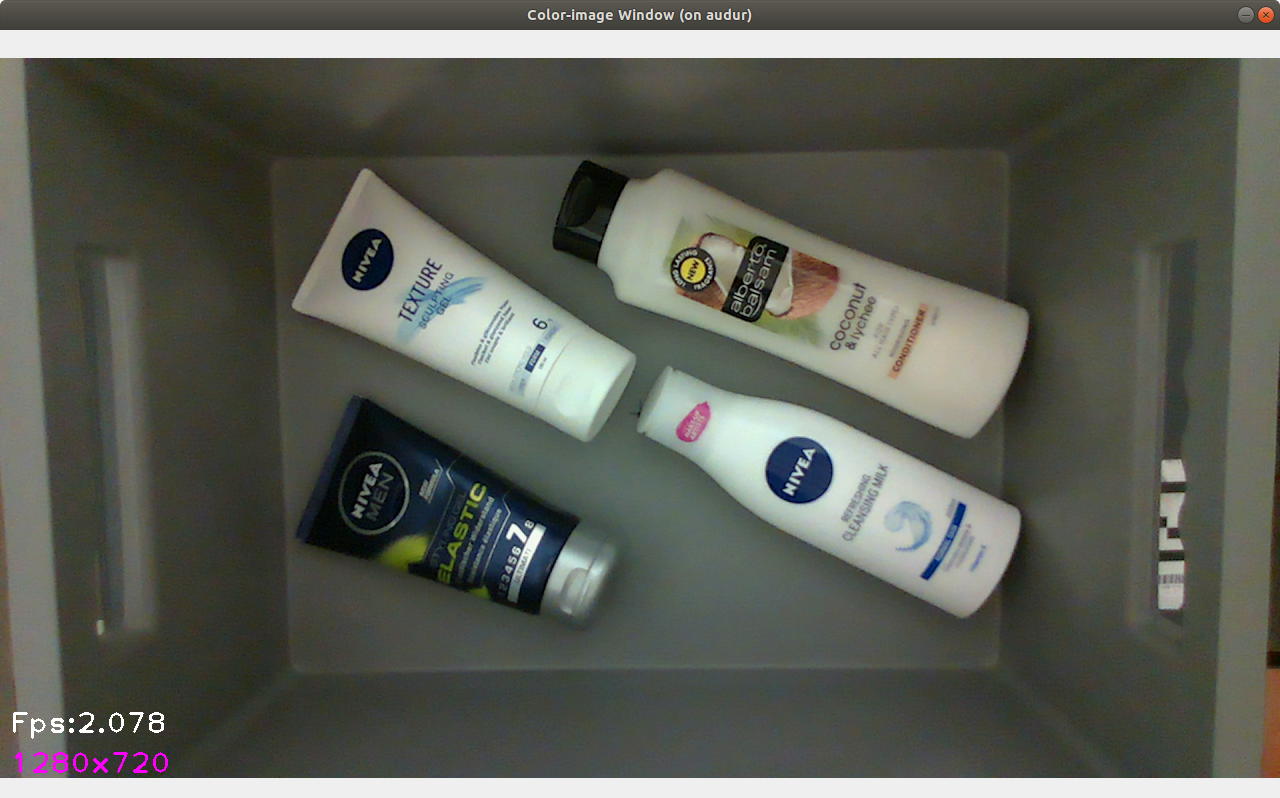
\includegraphics[width=0.3\textwidth, trim={0 0.6cm 0 2cm},clip]{graphics/results/beforetraining1.png}}
 \hfill
 \subfloat[The prior model]{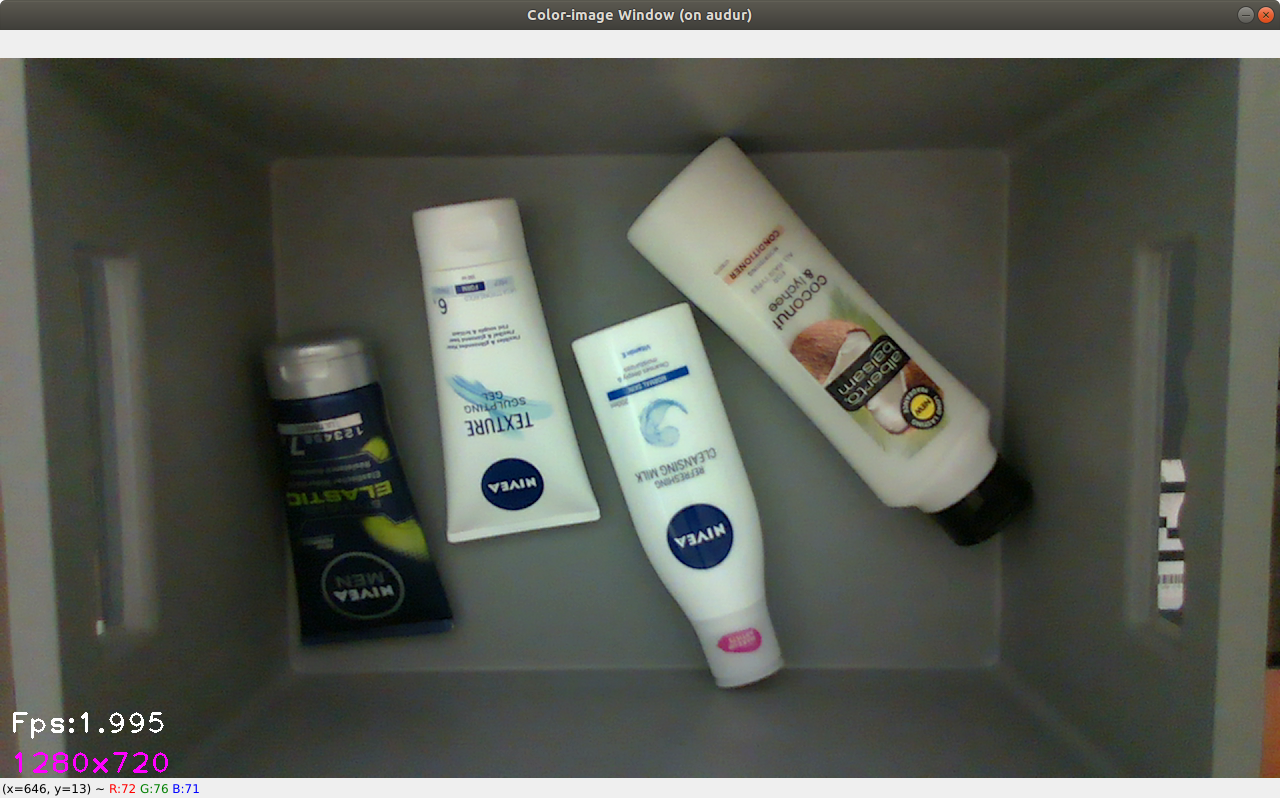
\includegraphics[width=0.3\textwidth, trim={0 0.6cm 0 2cm},clip]{graphics/results/beforetraining2.png}}
 \hfill \newline
 \subfloat[The posterior model]{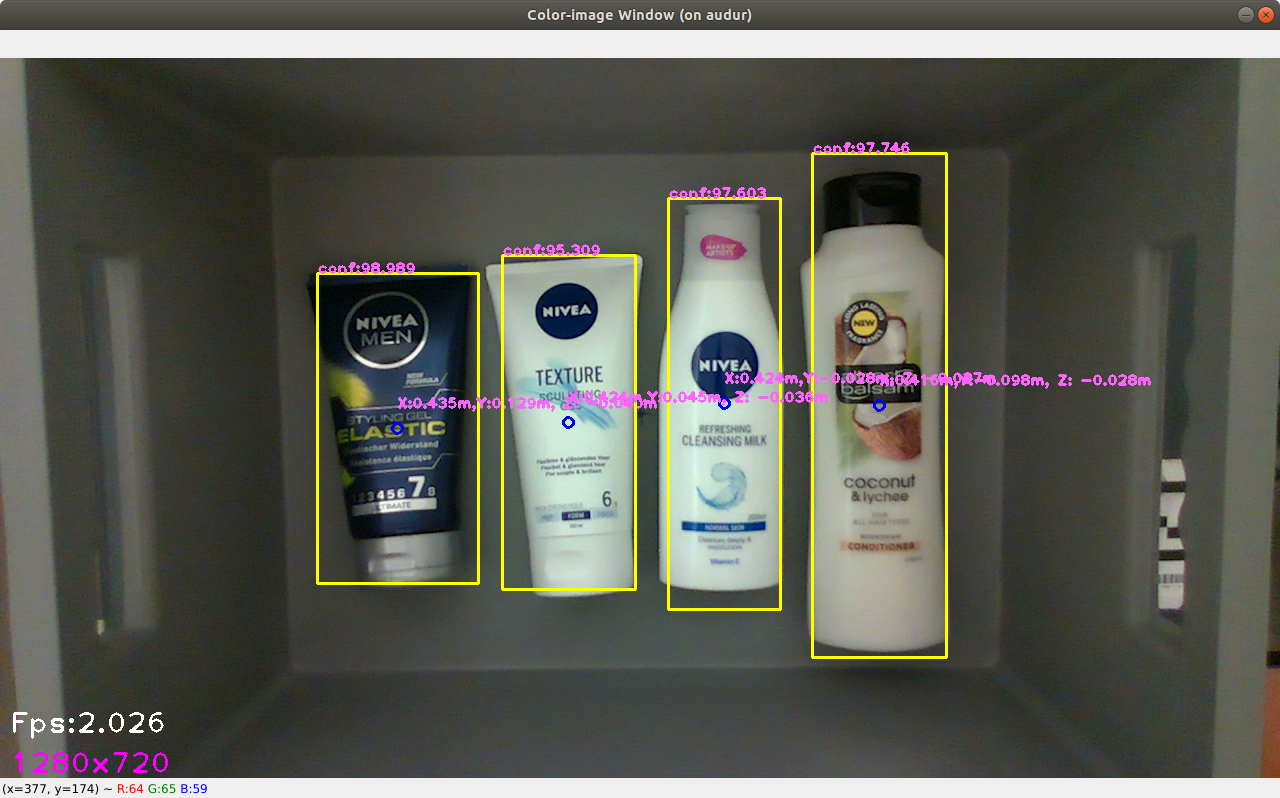
\includegraphics[width=0.3\textwidth, trim={0 0.6cm 0 2cm},clip]{graphics/results/aftertraining.png}}
 \hfill
 \subfloat[The posterior model]{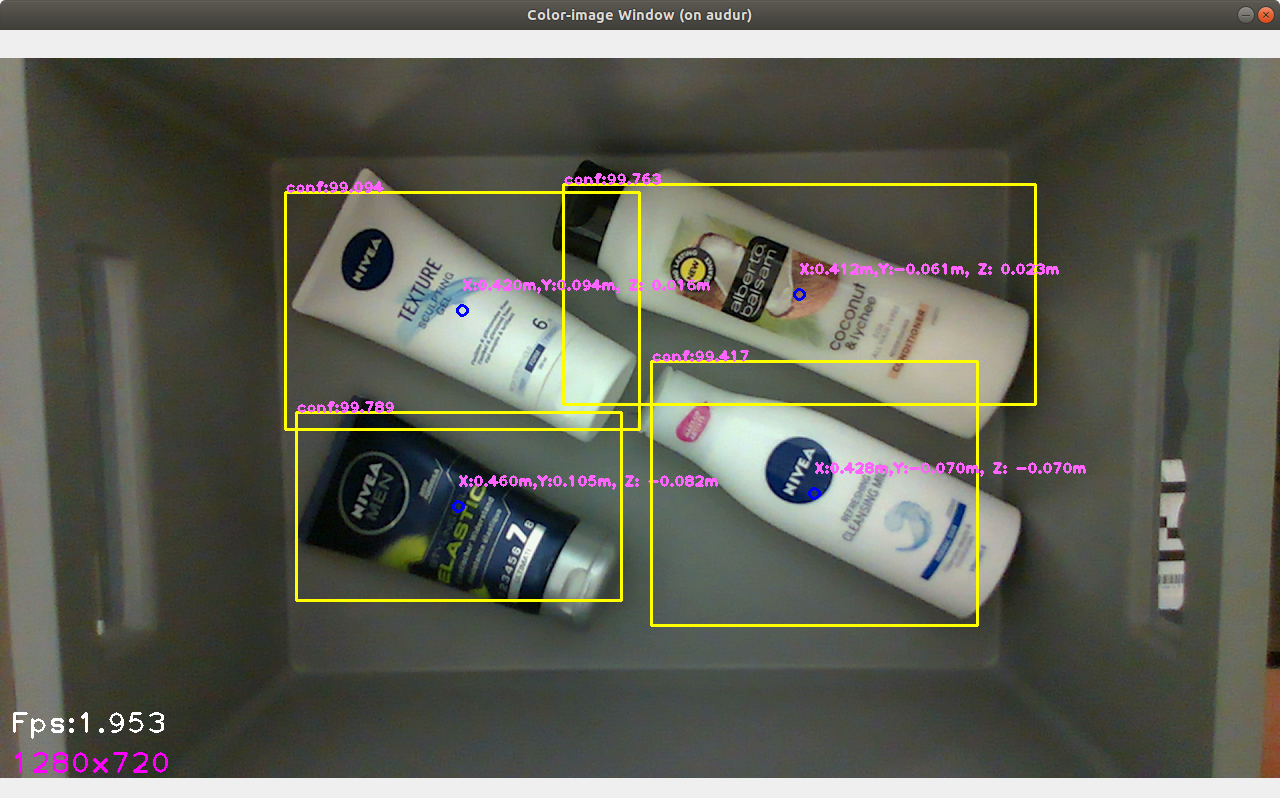
\includegraphics[width=0.3\textwidth, trim={0 0.6cm 0 2cm},clip]{graphics/results/aftertraining1.png}}
 \hfill
 \subfloat[The posterior model]{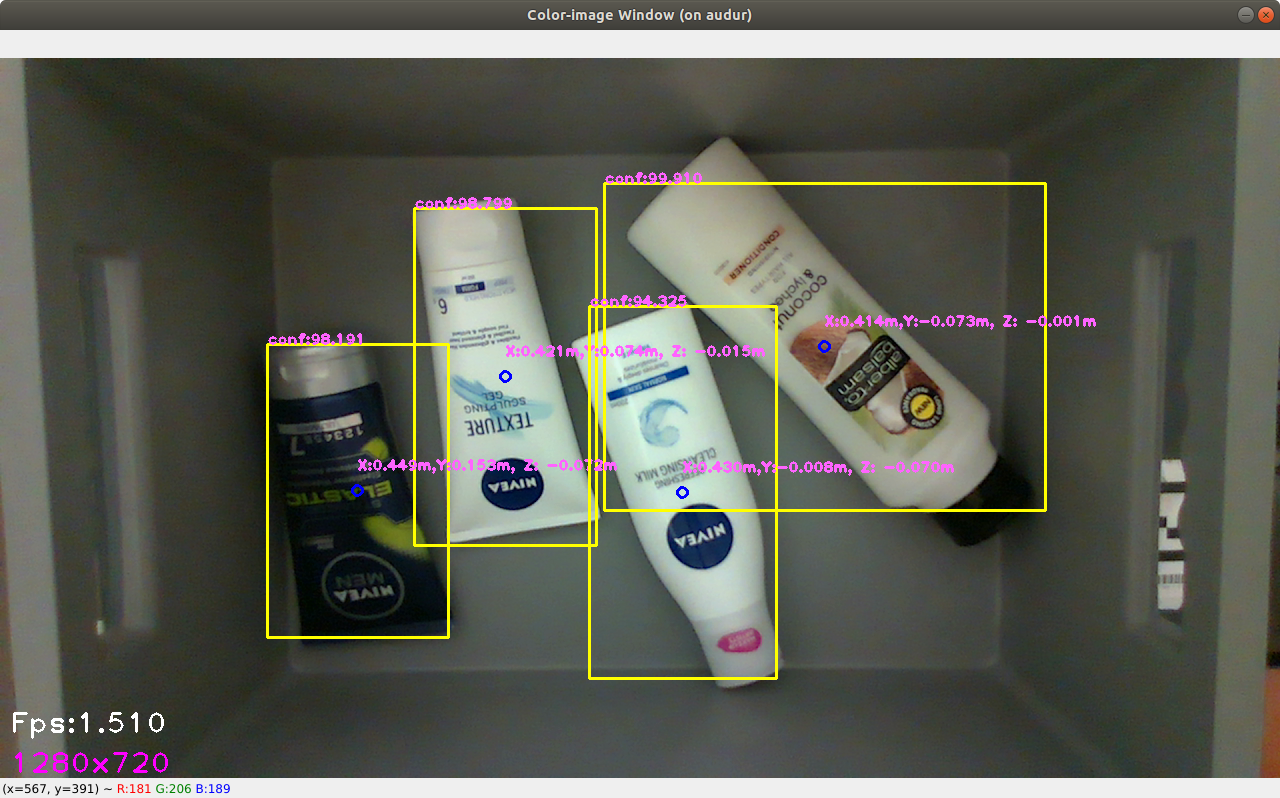
\includegraphics[width=0.3\textwidth, trim={0 0.6cm 0 2cm},clip]{graphics/results/aftertraining2.png}}
 \caption{The prior model trained on the COCO dataset and the posterior model trained on the robot generated dataset by transfer learning, starting from the weights of the prior model.}
 \label{figure: beforeaftertraining}
\end{figure}
\textit{Figure \ref{figure: beforeaftertraining}} shows visually how the performance changed before and after training, images in top row shows the results from the prior model trained on the COCO dataset and images in the bottom row shows the results from the first neural network that was trained on these products.

\pagebreak
\subsubsection{Single known items}\label{sec:resontrained}
\begin{figure}[h]
 \centering
 % include first image
 \subfloat[Alberto Balsam]{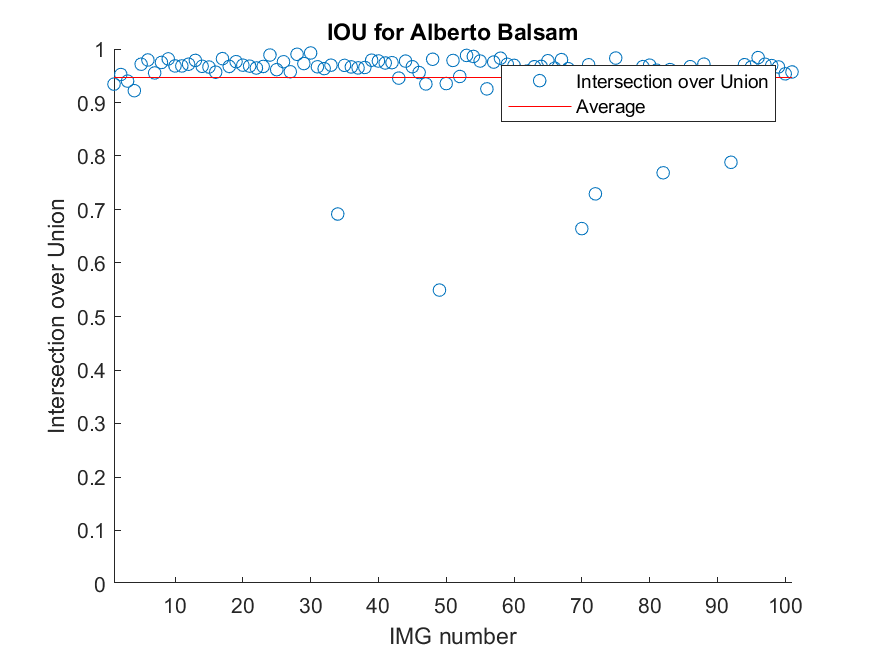
\includegraphics[width=0.5\textwidth, trim={0.6cm 0 0.6cm 0},clip]{graphics/results/albertobalsamIOU.png}}
 \hfill
 \subfloat[Nivea Cleansing Milk]{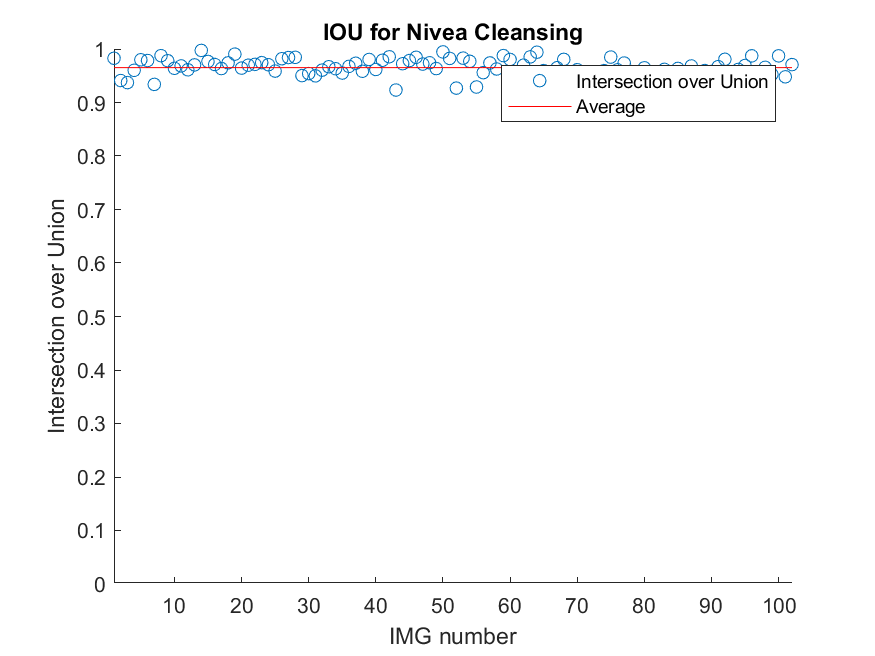
\includegraphics[width=0.5\textwidth, trim={0.6cm 0 0.6cm 0},clip]{graphics/results/niveacleansingIOU.png}}
 \hfill
 \subfloat[Nivea Elastic]{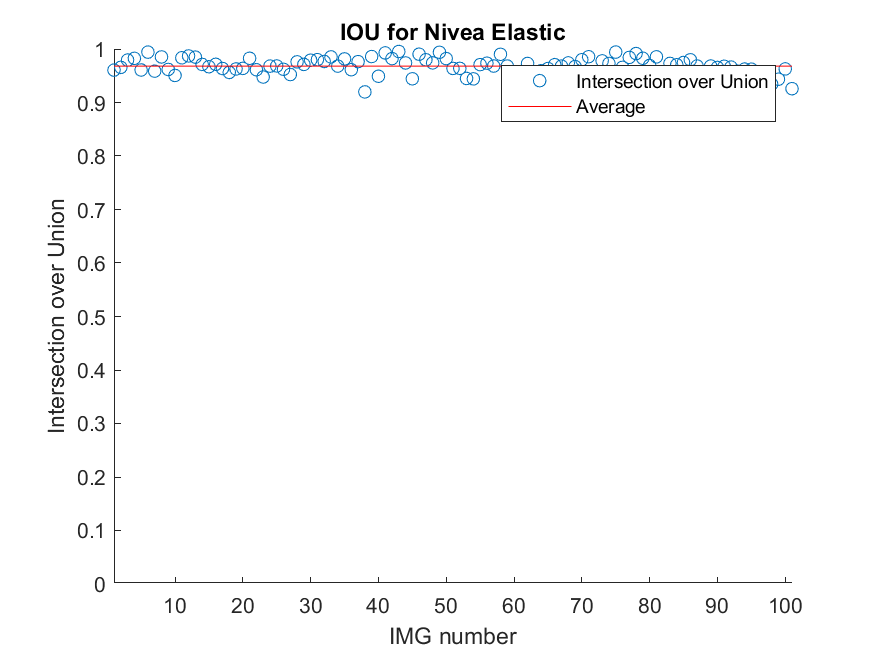
\includegraphics[width=0.5\textwidth, trim={0.6cm 0 0.6cm 0},clip]{graphics/results/niveaelasticIOU.png}}
 \hfill
 \subfloat[Nivea Texture]{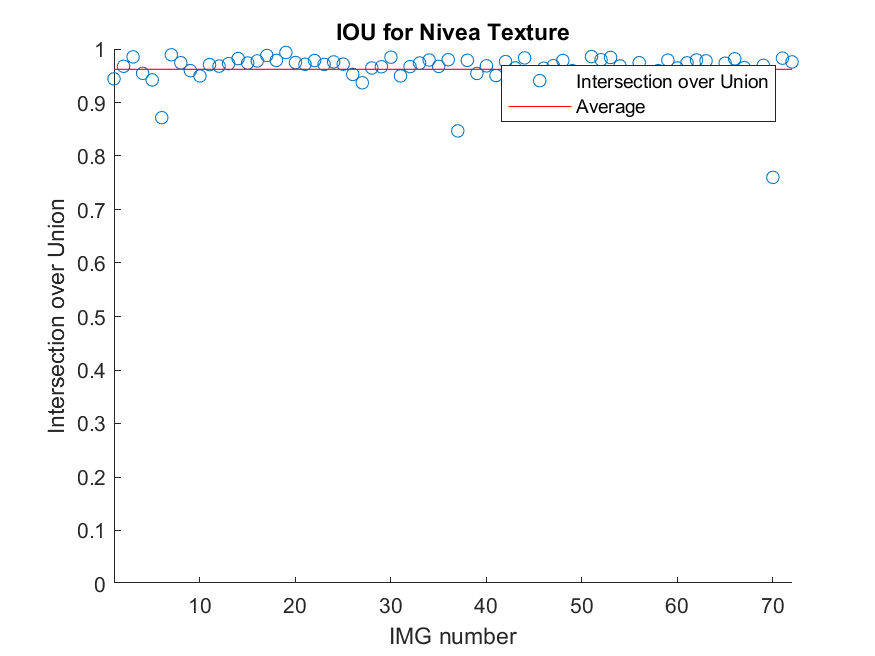
\includegraphics[width=0.5\textwidth, trim={0.6cm 0 0.6cm 0},clip]{graphics/results/niveatextureIOU.png}}
 \caption{Scatter plot for IoU on images of single items of known products}
 \label{figure: knownproducts}
\end{figure}
\textit{Figure \ref{figure: knownproducts}} shows raw IoU data from detection run on the training and test set from the first dataset \textit{(Sec: \ref{sec:firstdataset})}, it also shows an average IoU line on each scatter plot.

\begin{table}[h]
\resizebox{\textwidth}{!}{% 
\begin{tabular}{l|cccccccc}
\hline
\textit{Item} &
 \textit{Products} &
 \textit{Detections} &
 \textit{True Positive} &
 \textit{False Positive} &
 \textit{Avg-IoU} &
 \textit{Avg-Precision} &
 \textit{Avg-Recall} &
 \textit{Avg-F1} \\ \hline
Alberto Balsam & 101 & 101 & 101 & 0 & 0.9468 & 1 & 1 & 1 \\
Nivea C. Milk & 102 & 102 & 102 & 0 & 0.9652 & 1 & 1 & 1 \\
Nivea Elastic & 101 & 101 & 101 & 0 & 0.9679 & 1 & 1 & 1 \\
Nivea Texture & 72 & 72 & 72 & 0 & 0.9620 & 1 & 1 & 1 \\ \hline
\multicolumn{5}{r}{\textbf{Average:}} & \textit{0.9605} & \textit{1} & \textit{1} & \textit{1} 
\end{tabular}%
}
\caption{Detection results when tested on the training and test set from the first dataset \textit{(Sec: \ref{sec:firstdataset})} using the first neural network}
\label{tab:ready}
\end{table}

\textit{Table \ref{tab:ready}} shows the results applying the model on the training and test set from the first dataset \textit{(Sec: \ref{sec:firstdataset})}. When using the first trained neural network on images of single items of known products.
\clearpage

\begin{figure}[h]
 \centering
 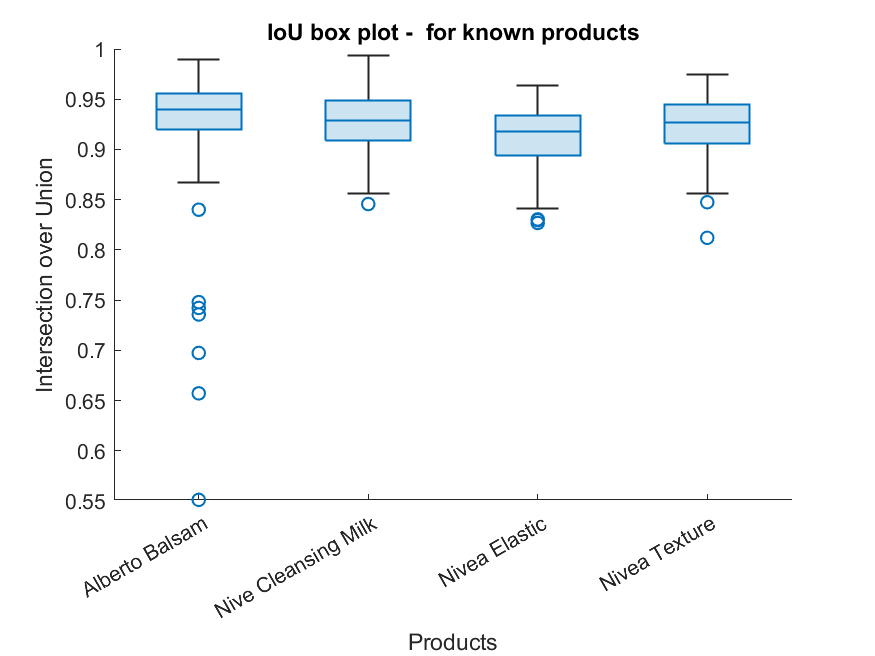
\includegraphics[width=0.8\textwidth]{graphics/results/boxplotForKnownProducts.png}
 \caption{Box plot for known products}
 \label{fig:boxknownproducts}
\end{figure}

\textit{Figure \ref{fig:boxknownproducts}} shows the IoU on 4 known products in a box plot when there is only one item in the bin. The ends of the box are the upper and lower quartiles, the vertical line inside the box is the median, and the bottom line is a lower extremity and the top line is an upper extreme. The Alberto Balsam has 6 extreme outliers points, the reason for that is there were 6 automatic labelled images of Alberto Balsam that didn’t have good annotation. 


\begin{figure}[h]
 \centering
 \subfloat[Highest IoU score]{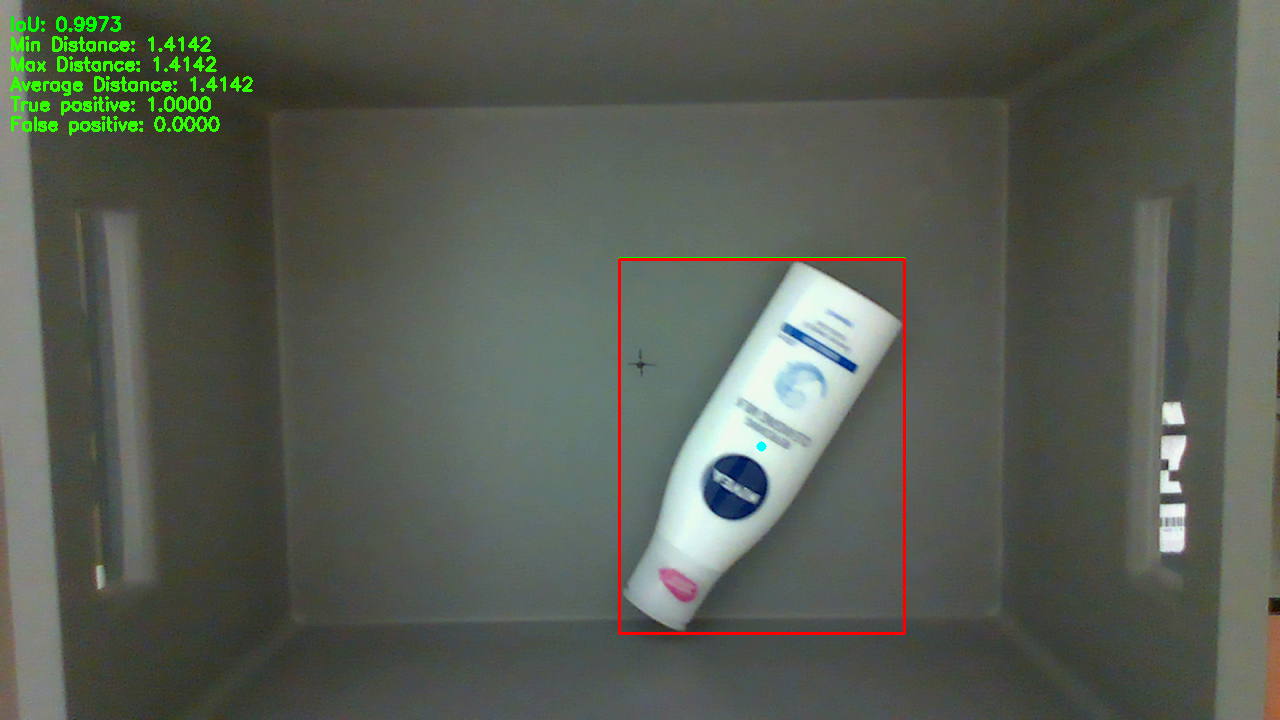
\includegraphics[width=0.5\textwidth]{graphics/results/v1Best.png}}
 \hfill
 \subfloat[Lowest IoU score]{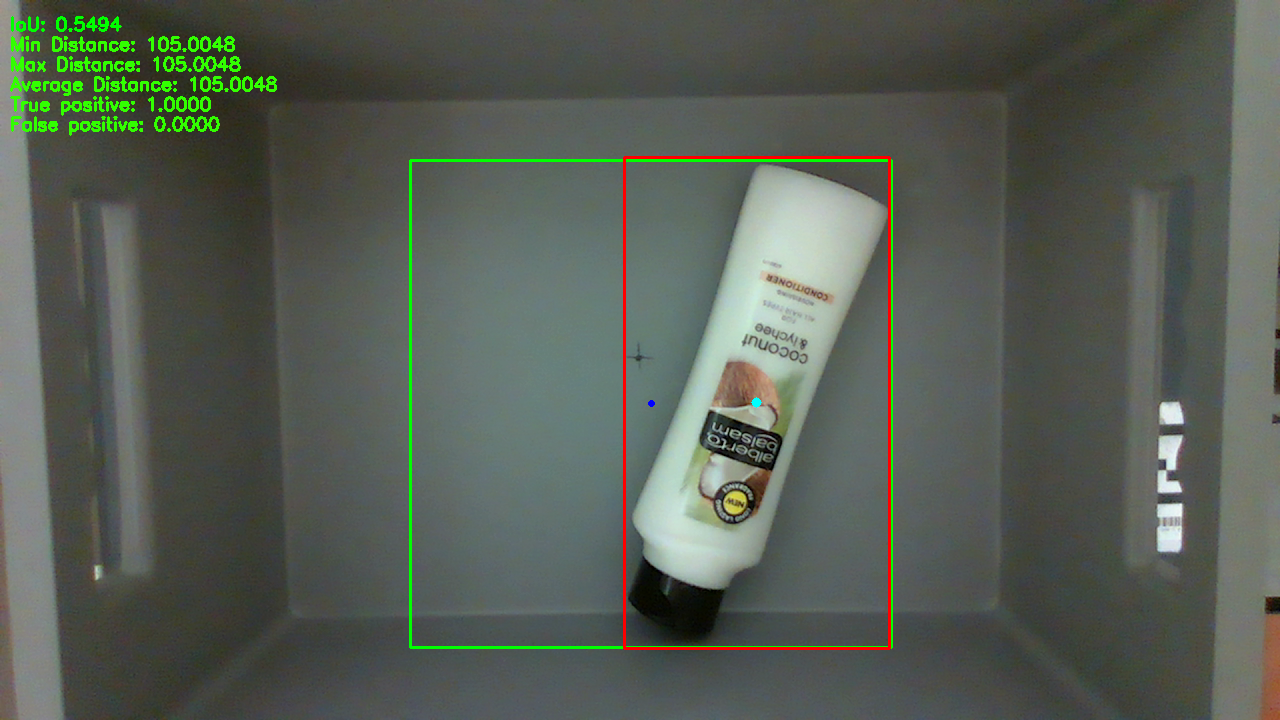
\includegraphics[width=0.5\textwidth]{graphics/results/v1Worst.png}\label{figure: v1worst}}
 \caption{Highest and lowest IoU score on the first neural network}
 \label{figure: v1bestworst}
\end{figure}

\textit{Figure \ref{figure: v1bestworst}} shows the highest and lowest IoU score on the first neural network when tested on the data set with one known item in the bin. The highest IoU score was 0.9973 and the lowest IoU score was 0.5494. The green bounding box is the automatically annotated bounding box and the red bounding box is the bounding box created by the neural network. In the example with the lowest IoU score, it can be seen that the neural network created a better bounding box than the bounding box that was created by the automatic labelling process.

\clearpage
\subsubsection{On unknown Beiersdorf products}\label{subsec:resunknownprod}
\begin{figure}[h]
 \centering
 % include first image
 \subfloat[Item 11]{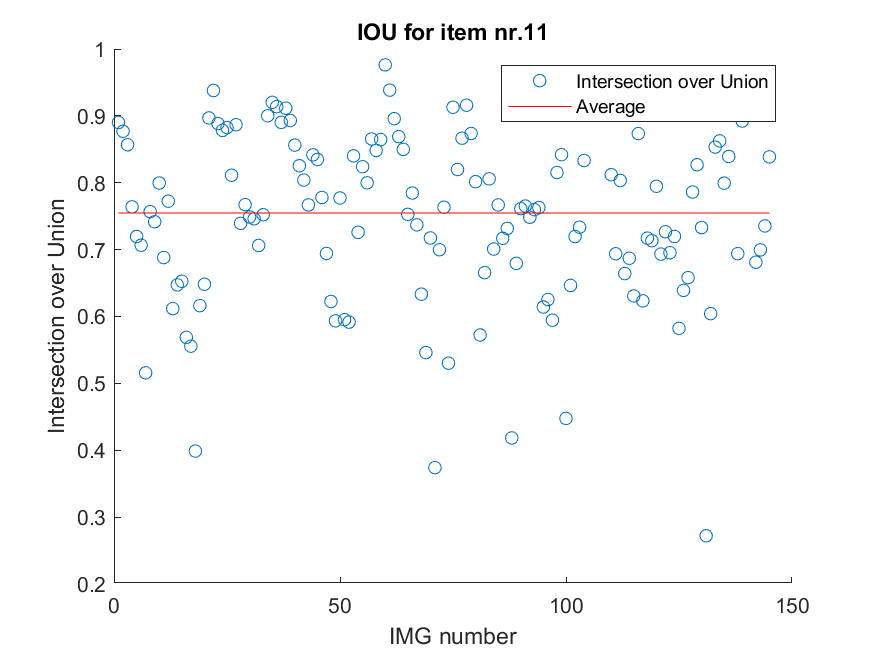
\includegraphics[width=0.5\textwidth, trim={0.6cm 0 0.6cm 0},clip]{graphics/results/item11.png}}
 \hfill
 % \subfloat[Item 12]{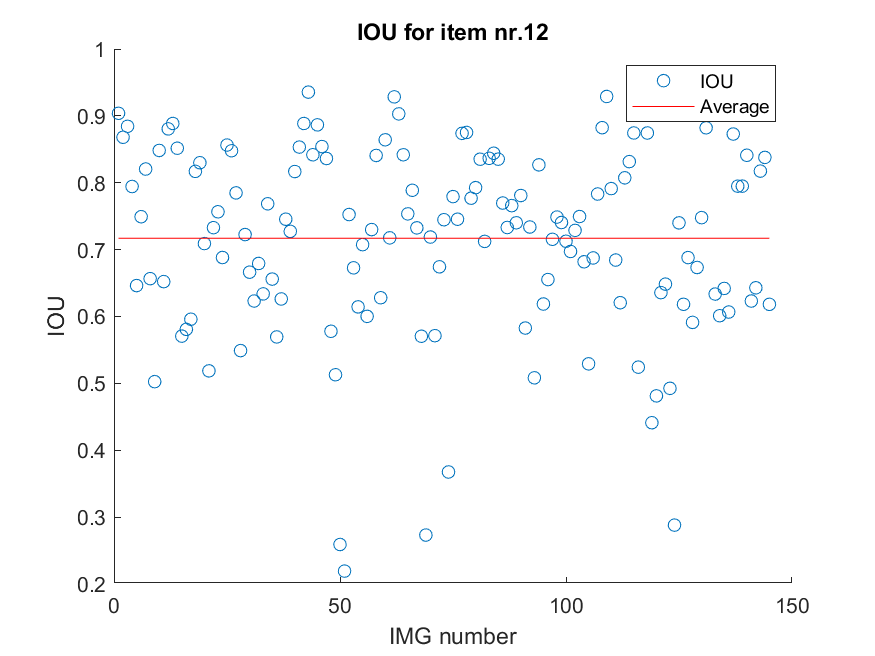
\includegraphics[width=0.245\textwidth]{graphics/results/item12.png}}
 % \hfill
 % \subfloat[Item 5]{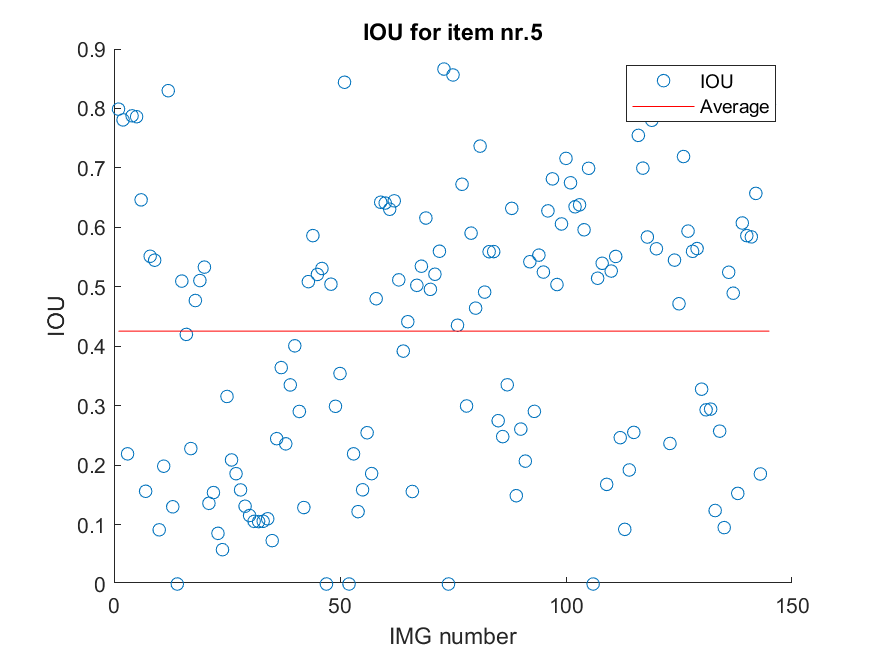
\includegraphics[width=0.245\textwidth]{graphics/results/item5.png}}
 % \hfill
 \subfloat[Item 6]{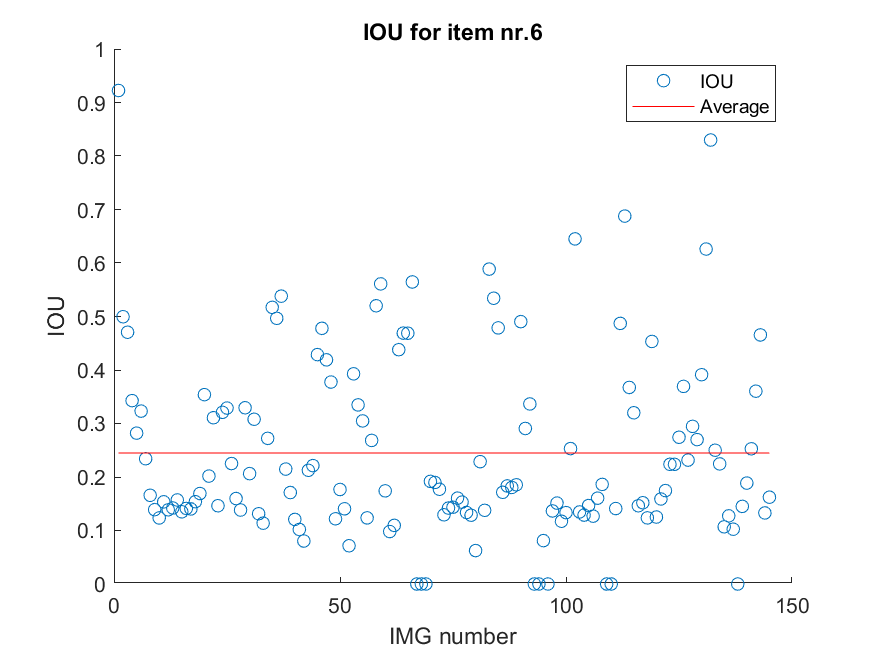
\includegraphics[width=0.5\textwidth, trim={0.6cm 0 0.6cm 0},clip]{graphics/results/item6.png}}
 \caption{Scatter plot for IoU on images of multiple items of unknown products}
 \label{figure: unknownproducts}
\end{figure}

\textit{Figure \ref{figure: unknownproducts}} shows raw IoU data from detection run on the Beiersdorf dataset \textit{(Sec: \ref{sec:beiersdorfdataset})}, it also shows an average IoU line on each scatter plot. The Beiersdorf data set has multiple unknown objects in the bin in each image.
Item nr. 11 had the highest average IoU or 0.7548 and item nr. 6 had the lowest average IoU or 0.2944. Raw data can be seen in the \textit{Appendix \ref{sec:apIoUresults}}.
% Please add the following required packages to your document preamble:
% \usepackage{graphicx}
\begin{table}[h]
\resizebox{\textwidth}{!}{%
\begin{tabular}{ccccccccc}
\hline
\multicolumn{1}{c|}{\textit{Item}} & \textit{Products} & \textit{Detections} & \textit{True Positive} & \textit{False Positive} & \textit{Avg-IoU} & \textit{Avg-Precision} & \textit{Avg-Recall} & \textit{Avg-F1} \\ \hline
\multicolumn{1}{c|}{1} & 684 & 361 & 334 & 24 & 0.6899 & 0.854 & 0.5479 & 0.6373 \\
\multicolumn{1}{c|}{2} & 1029 & 443 & 385 & 58 & 0.6123 & 0.7729 & 0.434 & 0.5231 \\
\multicolumn{1}{c|}{3} & 667 & 412 & 382 & 30 & 0.7145 & 0.877 & 0.6299 & 0.7087 \\
\multicolumn{1}{c|}{4} & 683 & 412 & 387 & 24 & 0.7246 & 0.8992 & 0.626 & 0.7068 \\
\multicolumn{1}{c|}{5} & 892 & 381 & 291 & 90 & 0.494 & 0.6533 & 0.3397 & 0.4317 \\
\multicolumn{1}{c|}{6} & 918 & 225 & 93 & 129 & 0.2944 & 0.2862 & 0.115 & 0.1588 \\
\multicolumn{1}{c|}{7} & 851 & 415 & 344 & 71 & 0.6008 & 0.7613 & 0.4117 & 0.5207 \\
\multicolumn{1}{c|}{8} & 788 & 362 & 339 & 23 & 0.7023 & 0.9182 & 0.4631 & 0.5893 \\
\multicolumn{1}{c|}{9} & 887 & 360 & 294 & 66 & 0.5417 & 0.7176 & 0.3551 & 0.46 \\
\multicolumn{1}{c|}{10} & 665 & 370 & 332 & 38 & 0.6625 & 0.8184 & 0.5293 & 0.6229 \\
\multicolumn{1}{c|}{11} & 627 & 407 & 386 & 21 & 0.7548 & 0.9264 & 0.6628 & 0.75 \\
\multicolumn{1}{c|}{12} & 574 & 453 & 431 & 20 & 0.7428 & 0.938 & 0.7891 & 0.8349 \\
\multicolumn{1}{c|}{13} & 618 & 329 & 320 & 9 & 0.745 & 0.9552 & 0.5786 & 0.6891 \\
\multicolumn{1}{c|}{14} & 1031 & 312 & 230 & 70 & 0.4798 & 0.6666 & 0.2746 & 0.3609 \\
\multicolumn{1}{c|}{15} & 616 & 330 & 310 & 18 & 0.7272 & 0.904 & 0.5607 & 0.6602 \\ \hline
\multicolumn{5}{r}{\textbf{Average:}} &\textit{ 0.6324} & \textit{0.7966} & \textit{0.4878} & \textit{0.5770}
\end{tabular}%
}
\caption{The results when tested on unknown data, using the first neural network}
\label{tab:test1unknown}
\end{table}

\textit{Table \ref{tab:test1unknown}} shows the results from the detection run on the Beiersdorf dataset \textit{(Sec: \ref{sec:beiersdorfdataset})} when using the trained first neural network on unknown products. As can be seen item nr. 12 has the best average precision, recall, and F-score.

% \begin{figure}[h]
% \centering
% 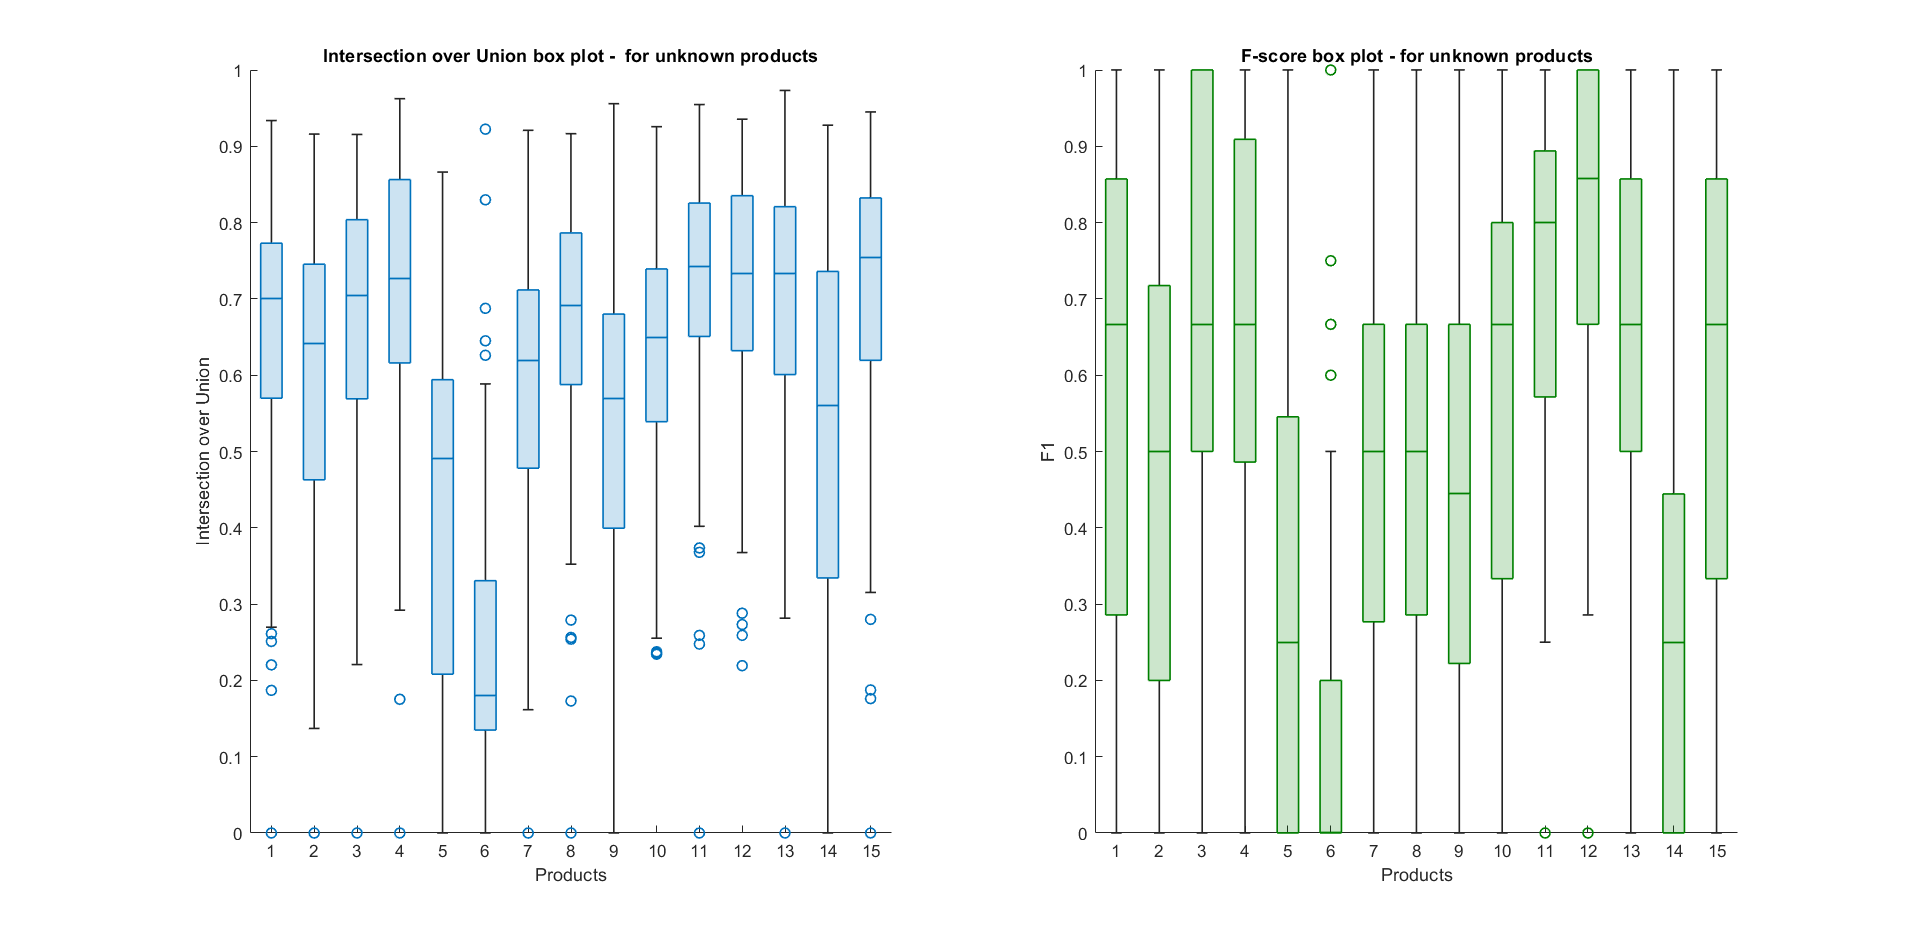
\includegraphics[width=1\textwidth, trim={8cm 0 8cm 0},clip]{graphics/results/boxplotForProducts.png}
% \caption{Box plot for unknown products, Intersection over Union on the left and F-score on the right}
% \label{fig:boxunknownproducts}
% \end{figure}
\clearpage

\begin{figure}[h]
 \centering
 % include first image
 \subfloat[Intersection over Union]{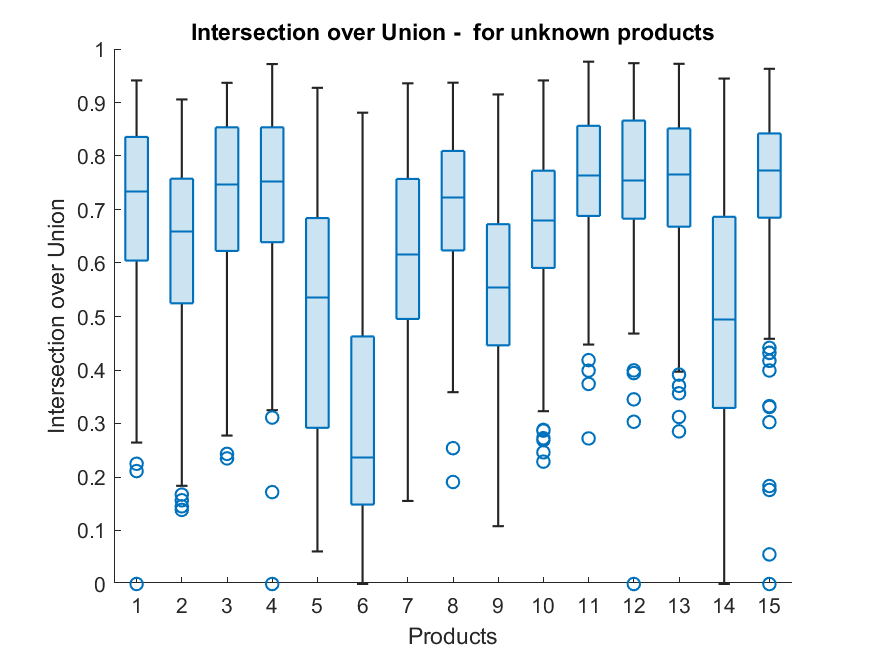
\includegraphics[width=0.5\textwidth, trim={0.5cm 0 1.5cm 0},clip]{graphics/results/iouboxplotForProducts.png}\label{fig:unknownioua}}
 \hfill
 \subfloat[F-score]{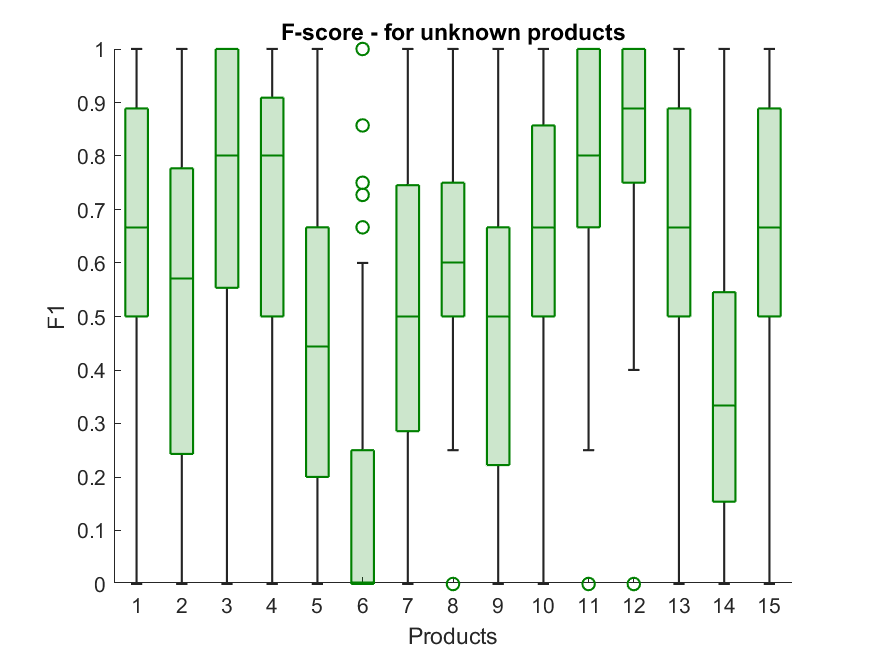
\includegraphics[width=0.5\textwidth, trim={0.5cm 0 1.5cm 0},clip]{graphics/results/f1boxplotForProducts.png}\label{fig:unknownioub}}
 
 \caption{Box plot on results for unknown products}
 \label{fig:unknowniou}
\end{figure}

\textit{Figure \ref{fig:unknowniou}} shows the IoU and F-score on 15 unknown products in a box plot when using the first neural network.
\begin{figure}[h]
 \centering
 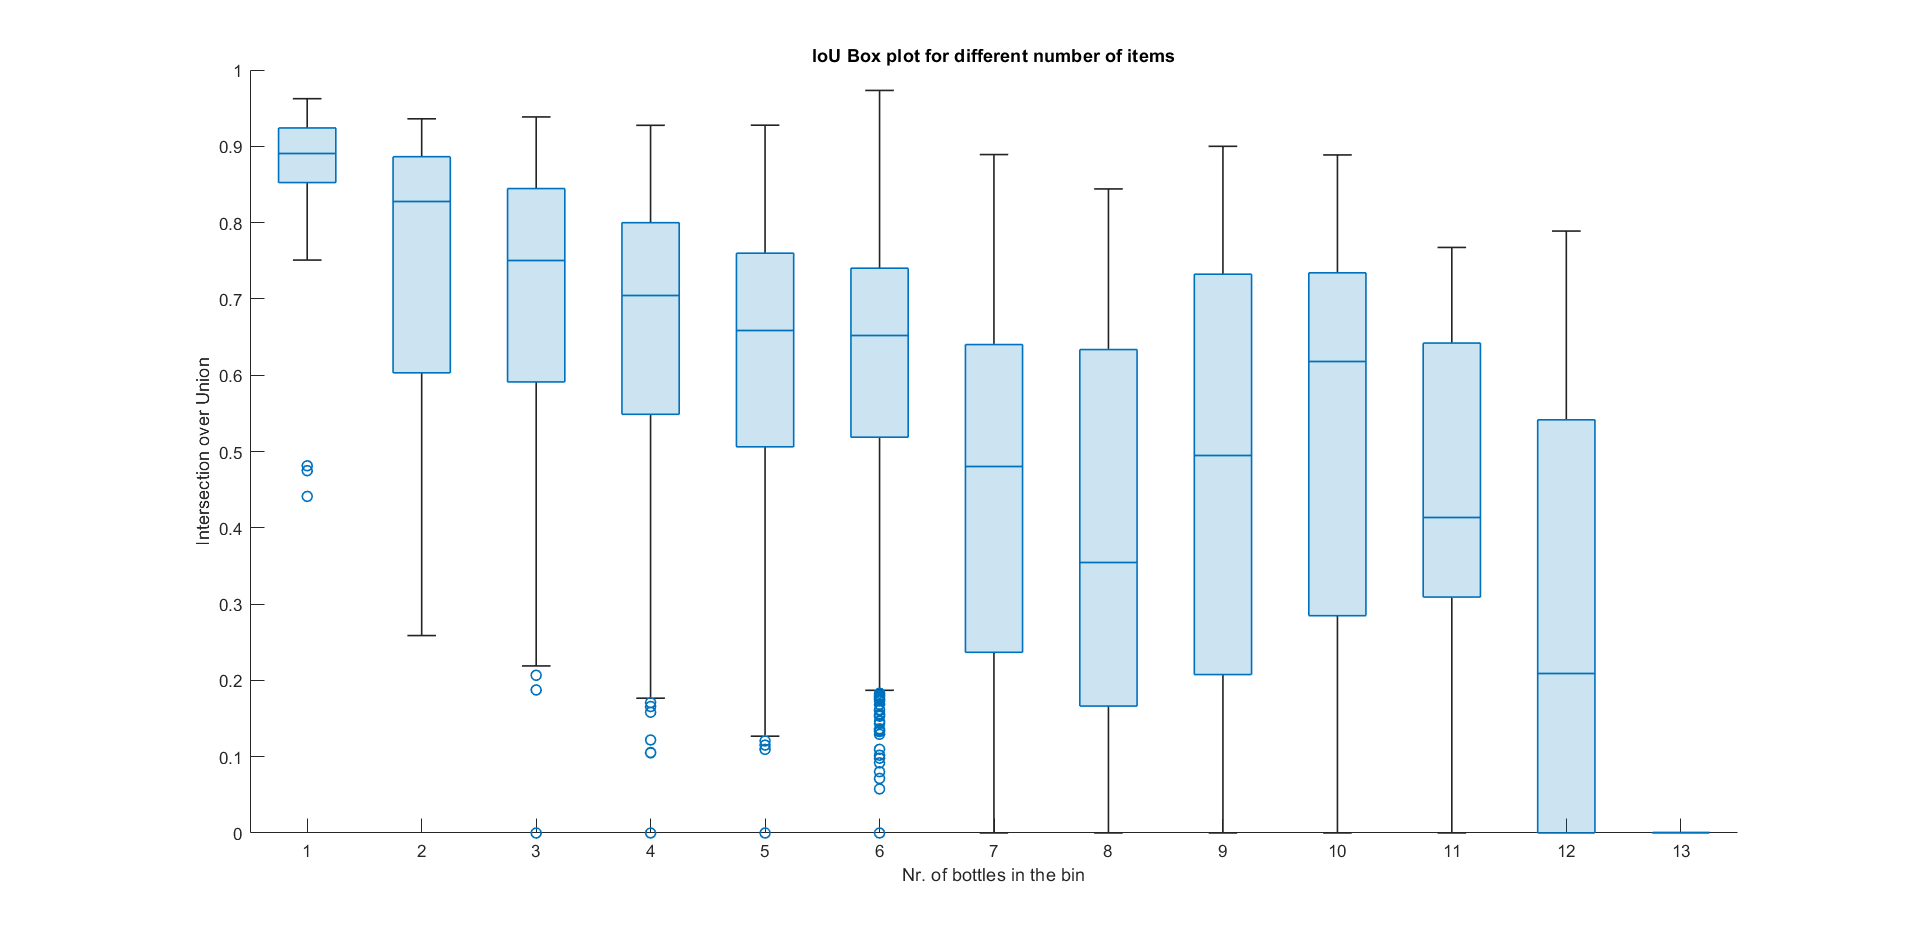
\includegraphics[width=0.9\textwidth]{graphics/results/boxplotBottles.png}
 \caption{IoU box plot for different number of items in the bin.}
 \label{fig:bottles}
\end{figure}

\textit{Figure \ref{fig:bottles}} shows also the IoU in the box plot, but for a different number of objects in the bin when using the first neural network. In this box plot, the X-axis is the number of bottles in the bin. The IoU has the highest IoU for single items and trends towards lower values as the number of items in the bin increases.
% You can point out to the reader that the IoU is highest for single items and trends towards lower values as the number of items in the bin increases. This is the plot to beat in the next experiment :-)]

\begin{figure}[h]
 \centering
 % include first image
 \subfloat[Highest IoU score, item nr. 11 ]{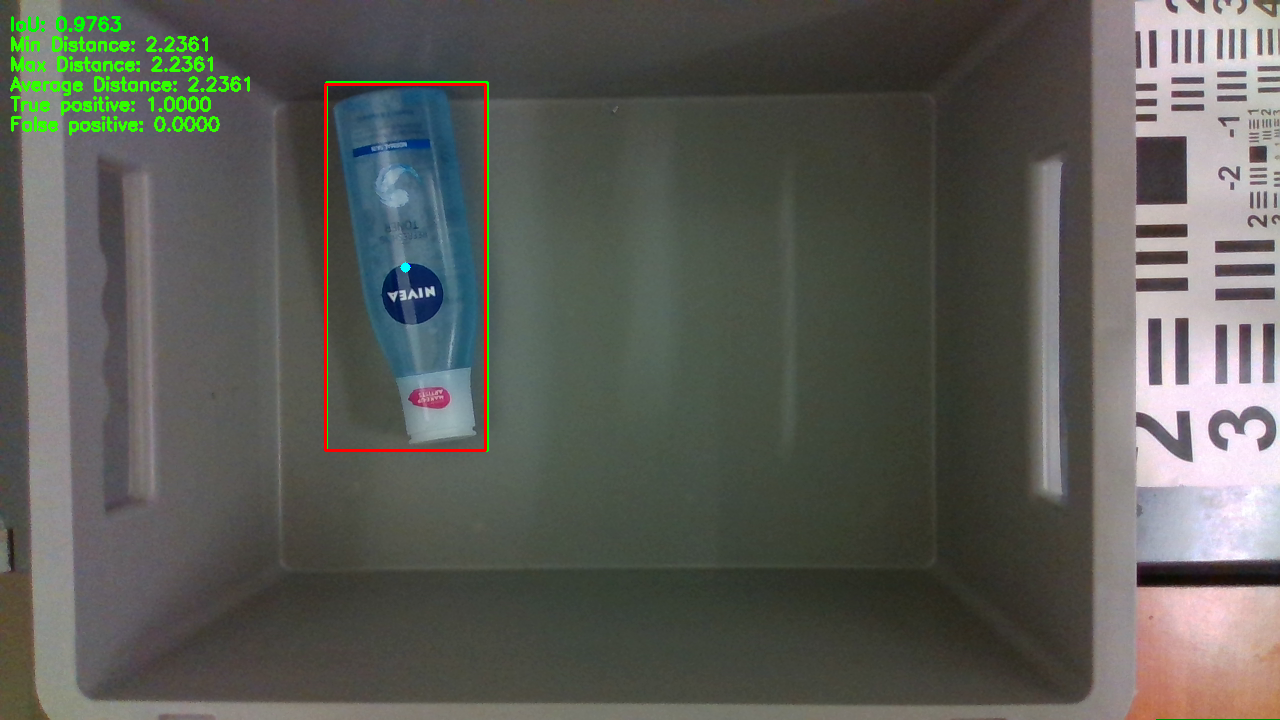
\includegraphics[width=0.5\textwidth]{graphics/results/v1best1.png}\label{fig:unknowniouaa}}
 \hfill
 \subfloat[Lowest IoU score, item nr. 6 ]{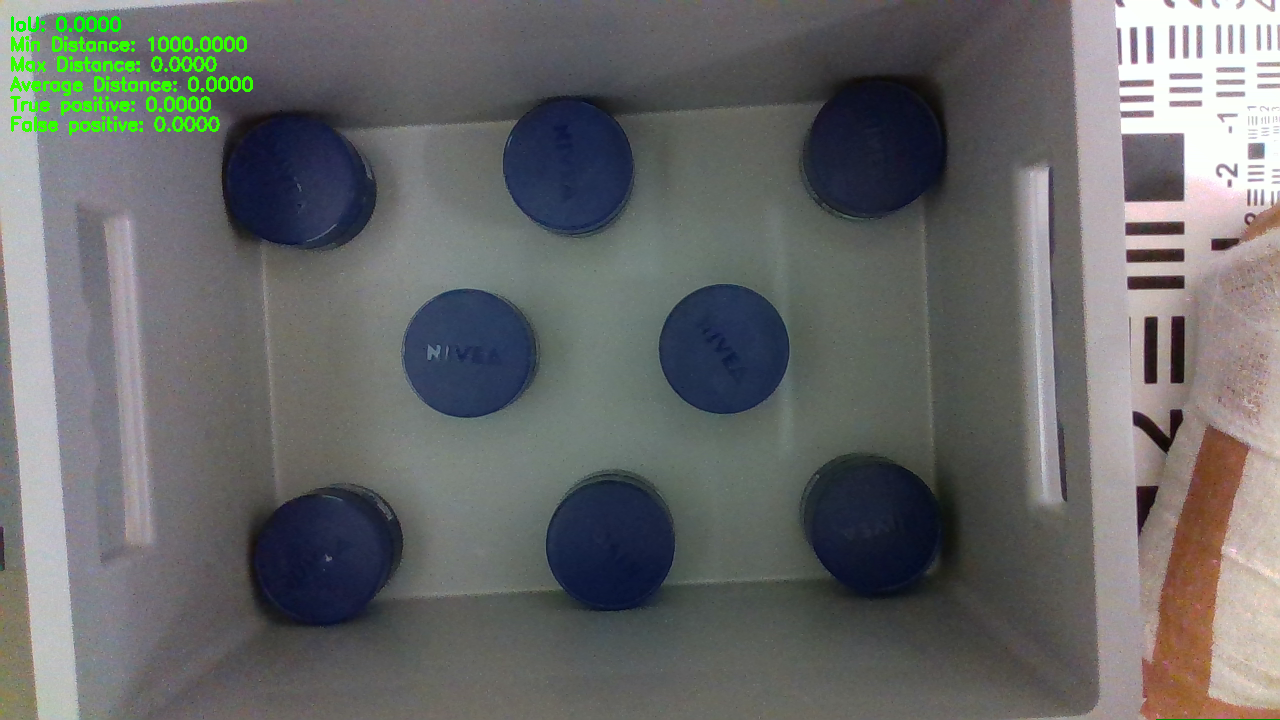
\includegraphics[width=0.5\textwidth]{graphics/results/v1worst1.png}\label{fig:unknownioubb}}
 
 \caption{Highest and lowest IoU score on the first neural network when testing on unknown items}
 \label{fig:v1unknowniou}
\end{figure}
\textit{Figure \ref{fig:v1unknowniou}} shows the highest and the lowest IoU score when using the first neural network on the Beiersdorf dataset, it can be seen that the highest IoU score is 0.9763 on item nr. 11 and the lowest IoU score is 0.00 on item nr 6.

\begin{figure}[h]
 \centering
 % include first image
 \subfloat[Highest True Positive detection, item nr. 9 ]{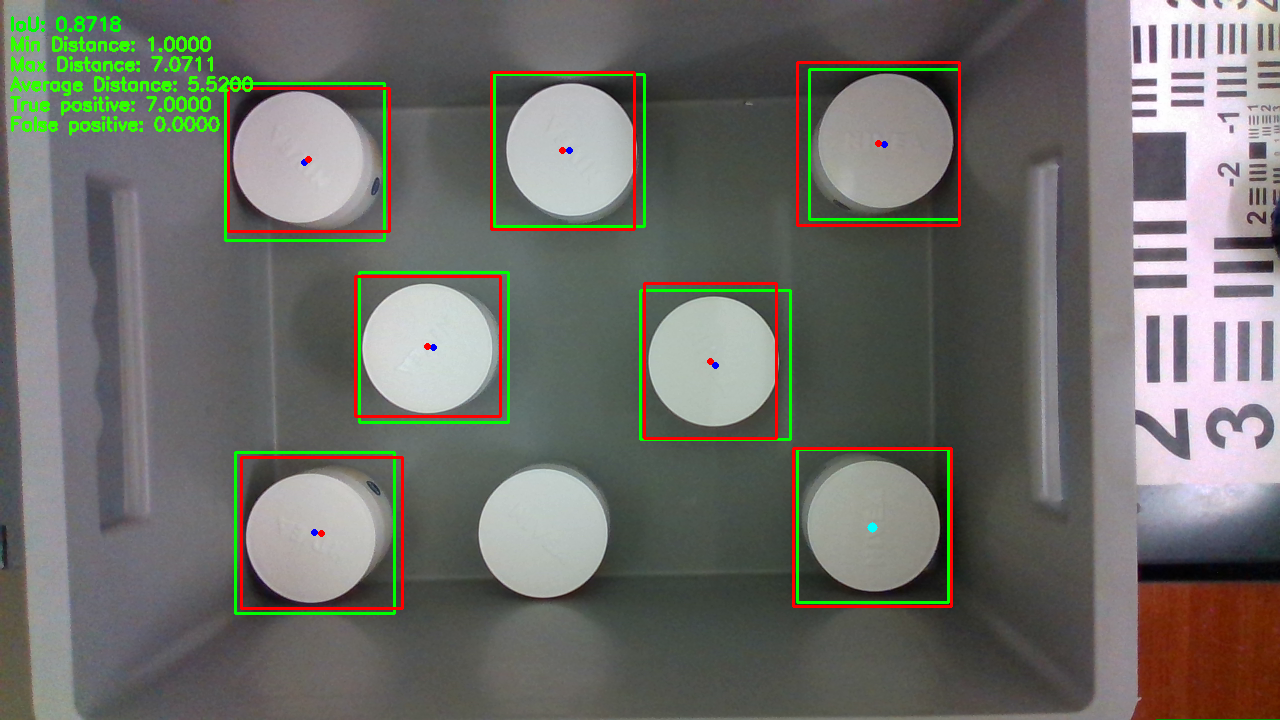
\includegraphics[width=0.5\textwidth]{graphics/results/ioumaxtrue.png}\label{fig:v1maxtrue}}
 \hfill
 \subfloat[Highest False Positive detection, item nr. 5 ]{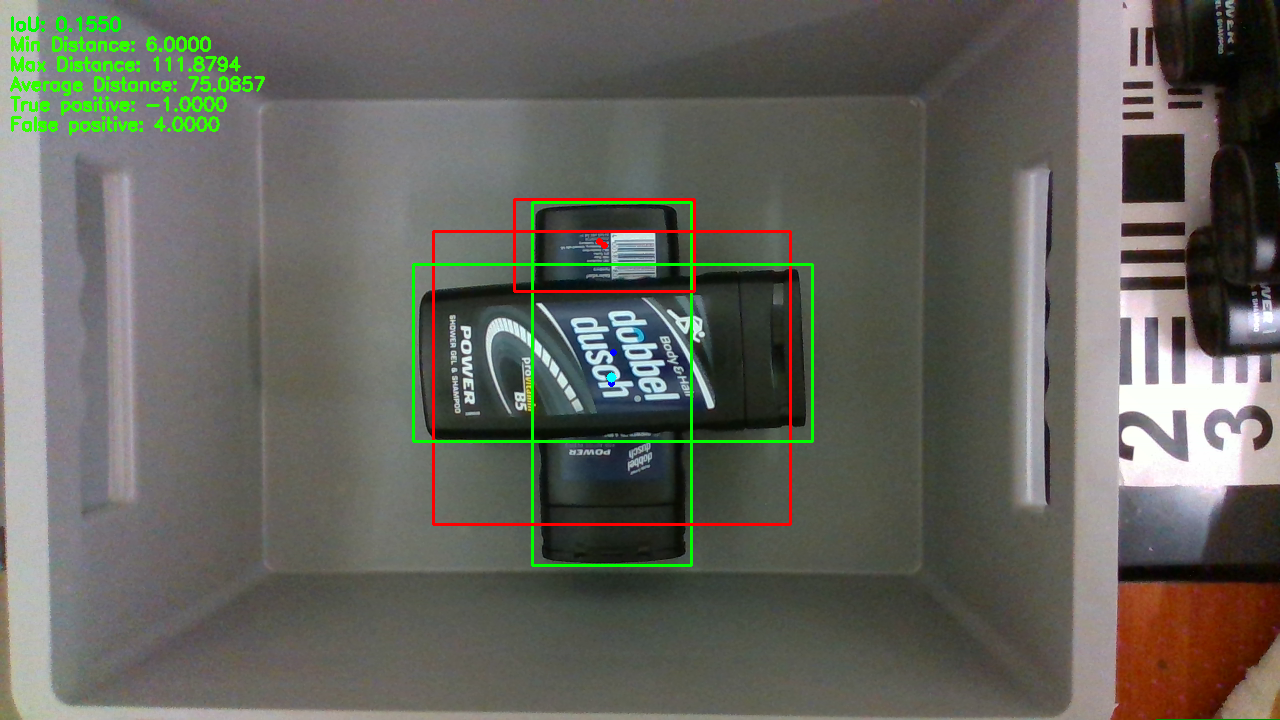
\includegraphics[width=0.5\textwidth]{graphics/results/ioumaxfalse.png}\label{fig:v1maxfalse}}
 
 \caption{Highest True and False Positive detection using the first neural network on unknown items}
 \label{fig:v1max}
\end{figure}
\textit{Figure \ref{fig:v1max}} shows the highest True Positive(TP) detection and the highest False Positive(FP) detection when using the first neural network on the Beiersdorf dataset, it can be seen that the highest TP is 7 objects and the highest FP is 4 objects.
\clearpage

\subsection{Results from the second neural network}\label{sec:secondneural}

\begin{figure}[h]
 \centering
 \includegraphics[width=0.8\textwidth, trim={5cm 0 4cm 0},clip]{graphics/results/secondneuralnetworkauto.png}
 \caption{IoU is measured over the test set on the automatically generated dataset with one object in the bin, every 1000 epochs}
 \label{fig:v2neuralnetwork}
\end{figure}
\textit{Figure \ref{fig:v2neuralnetwork}} shows how the IoU score developed over the number of epochs, when measuring over the test set. The best average IoU score can be seen in the red point and is 0.9546 at 37000 epochs. The average IoU is measured when running through the automatically generated dataset with one object in the bin(with both good and bad annotations).

%\fxfatal{skrifa meira setja inn mynd af því hvernig netið hegðar sér visually í bin eins og fyrsta neural}

\begin{figure}[h]
 \centering
 % include first image
 \subfloat[The prior model]{\includegraphics[width=0.33\textwidth, trim={0 0.6cm 0 2cm},clip ]{graphics/results/fullbinyolo-balsam.png}}
 \hfill
 \subfloat[The prior model]{\includegraphics[width=0.33\textwidth, trim={0 0.6cm 0 2cm},clip]{graphics/results/fullbinyolo-clean.png}}
 \hfill
 \subfloat[The prior model]{\includegraphics[width=0.33\textwidth, trim={0 0.6cm 0 2cm},clip]{graphics/results/fullbinyolo-elastic.png}}
 \hfill \newline
 \subfloat[The posterior model]{\includegraphics[width=0.33\textwidth, trim={0 0.6cm 0 2cm},clip]{graphics/results/fullbinv2-balsam.png}}
 \hfill
 \subfloat[The posterior model]{\includegraphics[width=0.33\textwidth, trim={0 0.6cm 0 2cm},clip]{graphics/results/fullbinv2-clean.png}}
 \hfill
 \subfloat[The posterior model]{\includegraphics[width=0.3\textwidth, trim={0 0.6cm 0 2cm},clip]{graphics/results/fullbinv2-elastic.png}}
 \caption{The prior model trained on the COCO dataset and the posterior model trained on the robot generated dataset by transfer learning, starting from the weights of the prior model.}
 \label{figure: v2beforeaftertraining}
\end{figure}
\textit{Figure \ref{figure: v2beforeaftertraining}} shows visually how the performance changed before and after training on bin full of objects, images in top row shows the results from the prior model trained on the COCO dataset and images in the bottom row shows the results from the second neural network that was trained on these products.

\clearpage
\subsubsection{Single known items} \label{sec:v2resontrained}
\begin{figure}[h]
 \centering
 % include first image
 \subfloat[Alberto Balsam]{\includegraphics[width=0.5\textwidth, trim={0.6cm 0 0.6cm 0},clip]{graphics/results/v2albertobalsamIOU.png}}
 \hfill
 \subfloat[Nivea Cleansing Milk]{\includegraphics[width=0.5\textwidth, trim={0.6cm 0 0.6cm 0},clip]{graphics/results/v2niveacleansingIOU.png}}
 \hfill
 \subfloat[Nivea Elastic]{\includegraphics[width=0.5\textwidth, trim={0.6cm 0 0.6cm 0},clip]{graphics/results/v2niveaelasticIOU.png}}
 \hfill
 \subfloat[Nivea Texture]{\includegraphics[width=0.5\textwidth, trim={0.6cm 0 0.6cm 0},clip]{graphics/results/v2niveatextureIOU.png}}
 \caption{Scatter plot for IoU on images of single items of known products} %Scatter plot for IoU on images of multiple items of unknown products
 \label{figure: v2knownproducts}
\end{figure}
\textit{Figure \ref{figure: v2knownproducts}} shows raw IoU data from detection run on the training and test set from the first dataset \textit{(Sec: \ref{sec:firstdataset})}, it also shows an average IoU line on each scatter plot.

\begin{table}[h]
\resizebox{\textwidth}{!}{% 
\begin{tabular}{l|cccccccc}
\hline
\textit{Item} &
 \textit{Products} &
 \textit{Detections} &
 \textit{True Positive} &
 \textit{False Positive} &
 \textit{Avg-IoU} &
 \textit{Avg-Precision} &
 \textit{Avg-Recall} &
 \textit{Avg-F1} \\ \hline
Alberto Balsam & 101 & 101 & 101 & 0 & 0.9512 & 1 & 1 & 1 \\
Nivea C. Milk & 102 & 102 & 102 & 0 & 0.9627 & 1 & 1 & 1 \\
Nivea Elastic & 101 & 101 & 101 & 0 & 0.9635 & 1 & 1 & 1 \\
Nivea Texture & 72 & 72 & 72 & 0 & 0.9575 & 1 & 1 & 1 \\ \hline
\multicolumn{5}{r}{\textbf{Average:}} & \textit{0.9587} & \textit{1} & \textit{1} & \textit{1} 
\end{tabular}%
}
\caption{Detection results when tested on trained data using the second neural network}
\label{tab:v2ready}
\end{table}
\textit{Table \ref{tab:v2ready}} shows the results from the detection run on the first dataset \textit{(Sec: \ref{sec:firstdataset})} when using the second trained neural network on images of single items of known products.

\clearpage
\begin{figure}[h]
 \centering
 \includegraphics[width=0.8\textwidth]{graphics/results/v2boxplotForKnownProducts.png}
 \caption{Box plot for known products}
 \label{fig:v2boxknownproducts}
\end{figure}
\textit{Figure \ref{fig:v2boxknownproducts}} shows the IoU on 4 known products in a box plot when there is only one item in the bin. The ends of the box are the upper and lower quartiles, the vertical line inside the box is the median, and the bottom line is a lower extremity and the top line is an upper extreme. The Alberto Balsam has 4 extreme outliers points, the reason for that is there were 6 automatic labelled images of Alberto Balsam that didn’t have good annotation. 

\begin{figure}[h]
 \centering
 \subfloat[Highest IoU score]{\includegraphics[width=0.5\textwidth]{graphics/results/v2Best.png}}
 \hfill
 \subfloat[Lowest IoU score]{\includegraphics[width=0.5\textwidth]{graphics/results/v2Worst.png}}
 \caption{Highest and lowest IoU score on the second neural network}
 \label{figure: v2bestworst}
\end{figure}

\textit{Figure \ref{figure: v2bestworst}} shows the highest and lowest IoU score on the second neural network when tested on the data set with one known item in the bin. The highest IoU score was 0.9974 and the lowest IoU score was 0.6730. The green bounding box is the automatically annotated bounding box and the red bounding box is the bounding box created by the second neural network.

\clearpage
\subsubsection{On unknown Beiersdorf products}\label{subsec:v2resunknownprod}

\begin{figure}[h]
 \centering
 % include first image
 \subfloat[Item 11]{\includegraphics[width=0.5\textwidth, trim={0.6cm 0 0.6cm 0},clip]{graphics/results/v2item11.png}}
 \hfill
 % \subfloat[Item 12]{\includegraphics[width=0.245\textwidth]{graphics/results/item12.png}}
 % \hfill
 % \subfloat[Item 5]{\includegraphics[width=0.245\textwidth]{graphics/results/item5.png}}
 % \hfill
 \subfloat[Item 6]{\includegraphics[width=0.5\textwidth, trim={0.6cm 0 0.6cm 0},clip]{graphics/results/v2item6.png}}
 \caption{Scatter plot for IoU on images of multiple items of unknown products}
 \label{figure: v2unknownproducts}
\end{figure}

\textit{Figure \ref{figure: v2unknownproducts}} shows raw IoU data from detection run on the Beiersdorf dataset \textit{(Sec: \ref{sec:beiersdorfdataset})}, it also shows an average IoU line on each scatter plot. The Beiersdorf data set has multiple items of unknown objects in the bin in each image.
Item nr. 11 had the highest average IoU or 0.7549 and item nr. 6 had the lowest average IoU or 0.2456. 

% Please add the following required packages to your document preamble:
% \usepackage{graphicx}
% Please add the following required packages to your document preamble:
% \usepackage{graphicx}
\begin{table}[h]
\resizebox{\textwidth}{!}{%
\begin{tabular}{c|cccccccc}
\hline
\textit{Item} &
 \textit{Products} &
 \textit{Detections} &
 \textit{True Positive} &
 \textit{False Positive} &
 \textit{Avg-IoU} &
 \textit{Avg-Precision} &
 \textit{Avg-Recall} &
 \textit{Avg-F1} \\ \hline
1 & 684 & 375 & 359 & 16 & 0.7106 & 0.9090 & 0.5840 & 0.6806 \\
2 & 1029 & 481 & 417 & 64 & 0.6008 & 0.7789 & 0.4641 & 0.5521 \\
3 & 667 & 413 & 385 & 28 & 0.7035 & 0.8810 & 0.6316 & 0.7135 \\
4 & 683 & 436 & 415 & 21 & 0.7272 & 0.9220 & 0.6599 & 0.7368 \\
5 & 892 & 262 & 175 & 87 & 0.4454 & 0.5408 & 0.2092 & 0.2891 \\
6 & 918 & 174 & 45 & 129 & 0.2456 & 0.1678 & 0.0563 & 0.0814 \\
7 & 851 & 381 & 297 & 84 & 0.5894 & 0.7090 & 0.3575 & 0.4622 \\
8 & 788 & 400 & 374 & 26 & 0.6932 & 0.9040 & 0.5070 & 0.6284 \\
9 & 887 & 369 & 299 & 70 & 0.5326 & 0.7082 & 0.3670 & 0.4675 \\
10 & 665 & 386 & 355 & 31 & 0.6802 & 0.8552 & 0.5609 & 0.6577 \\
11 & 627 & 432 & 407 & 25 & 0.7549 & 0.9159 & 0.6920 & 0.7679 \\
12 & 574 & 451 & 437 & 14 & 0.7490 & 0.9582 & 0.7963 & 0.8481 \\
13 & 618 & 345 & 335 & 10 & 0.7314 & 0.9408 & 0.5938 & 0.6978 \\
14 & 1031 & 291 & 243 & 48 & 0.5510 & 0.7210 & 0.2878 & 0.3823 \\
15 & 616 & 333 & 315 & 18 & 0.7348 & 0.8943 & 0.5603 & 0.6584 \\ \hline
\textit{\textbf{Average:}} &
 \textit{\textbf{769}} &
 \textit{\textbf{369}} &
 \textit{\textbf{324}} &
 \textit{\textbf{45}} &
 \textit{\textbf{0.6300}} &
 \textit{\textbf{0.7871}} &
 \textit{\textbf{0.4885}} &
 \textit{\textbf{0.5749}} \\ \hline
\textit{\textbf{Total:}} &
 \textit{\textbf{11530}} &
 \textit{\textbf{5529}} &
 \textit{\textbf{4858}} &
 \textit{\textbf{671}} &
 \textbf{-} &
 \textbf{-} &
 \textbf{-} &
 \textbf{-} \\ \hline
\end{tabular}%
}
\caption{The results when tested on unknown data, using the second neural network}
\label{tab:test2unknown}
\end{table}
\textit{Table \ref{tab:test2unknown}} shows the results from the detection run on the Beiersdorf dataset \textit{(Sec: \ref{sec:beiersdorfdataset})} when using the trained second neural network on unknown products. As can be seen item nr. 12 has the best average precision, recall, and F-score.


\clearpage

\begin{figure}[h]
 \centering
 % include first image
 \subfloat[Intersection over Union]{\includegraphics[width=0.5\textwidth, trim={0.5cm 0 1.5cm 0},clip]{graphics/results/v2iouboxplotForProducts.png}\label{fig:v2unknownioua}}
 \hfill
 \subfloat[F-score]{\includegraphics[width=0.5\textwidth, trim={0.5cm 0 1.5cm 0},clip]{graphics/results/v2f1boxplotForProducts.png}\label{fig:v2unknownioub}}
 
 \caption{Box plot on results for unknown products}
 \label{fig:v2unknowniou}
\end{figure}

\textit{Figure \ref{fig:v2unknowniou}} shows the IoU and F-score on 15 unknown products in a box plot when using the second neural network.

\begin{figure}[h]
 \centering
 \includegraphics[width=0.8\textwidth]{graphics/results/v2boxplotBottles.png}
 \caption{IoU box plot for different number of items in the bin.}
 \label{fig:v2bottles}
\end{figure}

\textit{Figure \ref{fig:v2bottles}} shows also the IoU in the box plot, but for a different number of objects in the bin when using the second neural network. In this box plot, the X-axis is the number of bottles in the bin. The IoU has the highest IoU for single items and trends towards lower values as the number of items in the bin increases.

\clearpage
\begin{figure}[h]
 \centering
 % include first image
 \subfloat[Highest IoU score, item nr. 13 ]{\includegraphics[width=0.5\textwidth]{graphics/results/v2best1.png}\label{fig:v2unknowniouaa}}
 \hfill
 \subfloat[Lowest IoU score, item nr. 5]{\includegraphics[width=0.5\textwidth]{graphics/results/v2worst1.png}\label{fig:v2unknownioubb}}
 
 \caption{Highest and lowest IoU score on the second neural network when testing on unknown items}
 \label{fig:v2unknowniou2}
\end{figure}

\textit{Figure \ref{fig:v2unknowniou2}} shows the highest and the lowest IoU score when using the second neural network on the Beiersdorf dataset, it can be seen that the highest IoU score is 0.9862 on item nr. 13 and the lowest IoU score is 0.00 on item nr. 5.

\begin{figure}[h]
 \centering
 % include first image
 \subfloat[Highest True positive detection, item nr. 2 ]{\includegraphics[width=0.5\textwidth]{graphics/results/v2ioumaxtrue.png}\label{fig:v2maxtrue}}
 \hfill
 \subfloat[Highest False Positive detection, item nr. 9 ]{\includegraphics[width=0.5\textwidth]{graphics/results/v2ioumaxfalse.png}\label{fig:v2maxfalse}}
 
 \caption{Highest True and False Positive detection using the second neural network on unknown items}
 \label{fig:v2max}
\end{figure}

\textit{Figure \ref{fig:v2max}} shows the highest True Positive(TP) detection and the highest False Positive(FP) detection when using the second neural network on the Beiersdorf dataset, it can be seen that the highest TP is 7 objects and the highest FP is 4 objects.

\clearpage
\subsubsection{On unknown Beiersdorf products - one detection per image}\label{subsec:v2zero}
Since the neural network is trained on images with only one annotations per image, the data was changed so it would be possible to see how it performs finding just one item per image.
% Please add the following required packages to your document preamble:
% \usepackage{graphicx}
\begin{table}[h]
\resizebox{\textwidth}{!}{%
\begin{tabular}{c|cccccccc}
\hline
\textit{Item} &
 \textit{Products} &
 \textit{Detections} &
 \textit{True Positive} &
 \textit{False Positive} &
 \textit{Avg-IoU} &
 \textit{Avg-Precision} &
 \textit{Avg-Recall} &
 \textit{Avg-F1} \\ \hline
1 & 145 & 142 & 136 & 6 & 0.7256 & 0.9379 & 0.9379 & 0.9379 \\
2 & 145 & 145 & 126 & 19 & 0.6008 & 0.8690 & 0.8690 & 0.8690 \\
3 & 145 & 145 & 135 & 10 & 0.7035 & 0.9310 & 0.9310 & 0.9310 \\
4 & 145 & 145 & 140 & 5 & 0.7272 & 0.9655 & 0.9655 & 0.9655 \\
5 & 145 & 136 & 94 & 42 & 0.4749 & 0.6483 & 0.6483 & 0.6483 \\
6 & 145 & 135 & 37 & 98 & 0.2638 & 0.2552 & 0.2552 & 0.2552 \\
7 & 145 & 145 & 131 & 14 & 0.5894 & 0.9034 & 0.9034 & 0.9034 \\
8 & 145 & 145 & 140 & 5 & 0.6932 & 0.9655 & 0.9655 & 0.9655 \\
9 & 145 & 144 & 116 & 28 & 0.5363 & 0.8000 & 0.8138 & 0.8138 \\
10 & 145 & 145 & 131 & 14 & 0.6802 & 0.9034 & 0.9034 & 0.9034 \\
11 & 145 & 145 & 141 & 4 & 0.7549 & 0.9724 & 0.9724 & 0.9724 \\
12 & 145 & 144 & 143 & 1 & 0.7542 & 0.9862 & 0.9862 & 0.9862 \\
13 & 145 & 144 & 138 & 6 & 0.7365 & 0.9517 & 0.9517 & 0.9517 \\
14 & 145 & 135 & 113 & 22 & 0.5918 & 0.7793 & 0.7793 & 0.7793 \\
15 & 145 & 141 & 134 & 7 & 0.7556 & 0.9241 & 0.9241 & 0.9241 \\ \hline
\textit{\textbf{Average:}} &
 \textit{\textbf{145}} &
 \textit{\textbf{142}} &
 \textit{\textbf{124}} &
 \textit{\textbf{19}} &
 \textit{\textbf{0.6392}} &
 \textit{\textbf{0.8529}} &
 \textit{\textbf{0.8538}} &
 \textit{\textbf{0.8538}} \\ \hline
\textit{\textbf{Total:}} &
 \textit{\textbf{2175}} &
 \textit{\textbf{2136}} &
 \textit{\textbf{1855}} &
 \textit{\textbf{281}} &
 \textbf{-} &
 \textbf{-} &
 \textbf{-} &
 \textbf{-} \\ \hline
\end{tabular}%
}
\caption{The results when tested on unknown data, and assuming one detection per each image}
\label{tab:v2zero}
\end{table}
%

\textit{Table \ref{tab:v2zero}} shows the results from the detection run on the Beiersdorf dataset \textit{(Sec: \ref{sec:beiersdorfdataset})} when using the trained second neural network on unknown products, but images with zero detections are not used to calculate the IoU. %As can be seen item nr. 15 has the best average IoU and precision, but item nr. 12 has the best recall and F1.

\begin{figure}[h]
 \centering
 % include first image
 \subfloat[Intersection over Union]{\includegraphics[width=0.5\textwidth, trim={0.5cm 0 1.5cm 0},clip]{graphics/v2zeroioubox.png}\label{fig:v2zeroa}}
 \hfill
 % \subfloat[F-score]{\includegraphics[width=0.33\textwidth, trim={0.5cm 0 1.5cm 0},clip]{graphics/v2zerof1box.png}\label{fig:v2zerob}}
 % \hfill
 \subfloat[Intersection over Union for different number of items in the bin]{\includegraphics[width=0.5\textwidth, trim={0.5cm 0 1.5cm 0},clip]{graphics/v2zerobottles.png}\label{fig:v2zeroc}}
 
 \caption{Box plot on results for unknown products, when zero detections are eliminated}
 \label{fig:v2zerofig}
\end{figure}

\textit{Figure \ref{fig:v2zerofig}} shows the IoU and the IoU for a different number of items in the bin, on 15 unknown products in a box plot when using the second neural network.


\clearpage
%%%%%%%%%%%%%%%%%%%%%%% Third neural network ------------------
\subsection{Results from the third neural network}
\begin{figure}[h]
 \centering
 \includegraphics[width=0.8\textwidth, trim={5cm 0 4cm 0},clip]{graphics/results/thirdneuralnetwork.png}
 \caption{IoU is measured over the test set on the automatically generated dataset with multiple objects in the bin, every 1000 epochs}
 \label{fig:v3neuralnetwork}
\end{figure}
\textit{Figure \ref{fig:v3neuralnetwork}} shows how the IoU score developed over the number of epochs when measuring over the test set. The best average IoU score on the test set can be seen in the red point and is 0.9067 at 22000 epochs. The average IoU is measured when running through the automatically generated dataset with multiple objects in the bin.

%\fxfatal{Skrifa þegar ég fæ result ur þvi}

\begin{figure}[h]
 \centering
 % include first image
 \subfloat[Second neural network]{\includegraphics[width=0.33\textwidth, trim={0 0.6cm 0 2cm},clip ]{graphics/results/v2-1.png}}
 \hfill
 \subfloat[Second neural network]{\includegraphics[width=0.33\textwidth, trim={0 0.6cm 0 2cm},clip]{graphics/results/v2-2.png}}
 \hfill
 \subfloat[Second neural network]{\includegraphics[width=0.33\textwidth, trim={0 0.6cm 0 2cm},clip]{graphics/results/v2-3.png}}
 \hfill \newline
 \subfloat[Third neural network]{\includegraphics[width=0.33\textwidth, trim={0 0.6cm 0 2cm},clip]{graphics/results/v3-1.png}}
 \hfill
 \subfloat[Third neural network]{\includegraphics[width=0.33\textwidth, trim={0 0.6cm 0 2cm},clip]{graphics/results/v3-2.png}}
 \hfill
 \subfloat[Third neural network]{\includegraphics[width=0.33\textwidth, trim={0 0.6cm 0 2cm},clip]{graphics/results/v3-3.png}}
 \caption{Second neural network and the posterior model (third neural network)}
 \label{figure: v3beforeaftertraining}
\end{figure}
\textit{Figure \ref{figure: v3beforeaftertraining}} shows visually how the performance changed from the second neural network (\textit{trained on automatically generated dataset with one object in the bin}) and third neural network (\textit{trained on automatically generated dataset with multiple objects in the bin}). 
\clearpage
\subsubsection{On multiple known items} \label{sec:v3resontrained}
\begin{figure}[h]
 \centering
 % include first image
 \subfloat[Alberto Balsam]{\includegraphics[width=0.5\textwidth, trim={0.6cm 0 0.6cm 0},clip]{graphics/results/v3albertobalsamIOU.png}}
 \hfill
 \subfloat[Nivea Cleansing Milk]{\includegraphics[width=0.5\textwidth, trim={0.6cm 0 0.6cm 0},clip]{graphics/results/v3niveacleansingIOU.png}}
 \hfill
 \subfloat[Nivea Elastic]{\includegraphics[width=0.5\textwidth, trim={0.6cm 0 0.6cm 0},clip]{graphics/results/v3niveaelasticIOU.png}}
 \hfill
 \subfloat[Nivea Texture]{\includegraphics[width=0.5\textwidth, trim={0.6cm 0 0.6cm 0},clip]{graphics/results/v3niveatextureIOU.png}}
 \caption{Scatter plot for IoU on images with multiple items of known products} %Scatter plot for IoU on images of multiple items of unknown products
 \label{figure: v3knownproducts}
\end{figure}
\textit{Figure \ref{figure: v3knownproducts}} shows raw IoU data from detection run on the training and test set from the dataset with multiple items in the bin\textit{(Sec: \ref{sec:multidataset})}, it also shows an average IoU line on each scatter plot.


% Please add the following required packages to your document preamble:
% \usepackage{graphicx}
\begin{table}[h]
\resizebox{\textwidth}{!}{%
\begin{tabular}{ccccccccc}
\hline
\multicolumn{1}{c|}{\textit{Item}} &
 \textit{Products} &
 \textit{Detections} &
 \textit{True Positive} &
 \textit{False Positive} &
 \textit{Avg-IoU} &
 \textit{Avg-Precision} &
 \textit{Avg-Recall} &
 \textit{Avg-F1} \\ \hline
\multicolumn{1}{c|}{1} & 16 & 19 & 11 & 8 & 0.6132 & 0.625 & 0.6875 & 0.6458 \\
\multicolumn{1}{c|}{2} & 11 & 11 & 8 & 1 & 0.6658 & 0.7273 & 0.7273 & 0.7273 \\
\multicolumn{1}{c|}{3} & 24 & 24 & 20 & 2 & 0.7839 & 0.8333 & 0.8333 & 0.8333 \\
\multicolumn{1}{c|}{4} & 19 & 20 & 14 & 3 & 0.7184 & 0.7368 & 0.7368 & 0.7368 \\ \hline
\multicolumn{5}{r}{\textbf{Average:}} & \textit{0.6953} & \textit{0.7306} & \textit{0.7462} & \textit{0.7358}
\end{tabular}%
}
\caption{Detection results when tested on trained data using the third neural network}
\label{tab:v3known}
\end{table}
\textit{Table \ref{tab:v3known}} shows the results from the detection run on the second dataset with multiple known items in the bin \textit{(Sec: \ref{sec:multidataset})} when using the third trained neural network. The IoU, Precision, Recall, and F1 are calculated for each image, and then an average is taken over each item. 

\begin{figure}[h]
 \centering
 \includegraphics[width=1\textwidth]{graphics/results/v3boxplotForKnownProducts.png}
 \caption{Box plot for known products}
 \label{fig:v3boxknownproducts}
\end{figure}
\textit{Figure \ref{fig:v3boxknownproducts}} shows the IoU on 4 known products in a box plot when there are multiple items in the bin. These results show that the third neural network is fragile on known items.

\begin{figure}[h]
 \centering
 \subfloat[Highest IoU score]{\includegraphics[width=0.45\textwidth]{graphics/results/v3best.png}}
 \hspace{0.5cm}
 \subfloat[Lowest IoU score]{\includegraphics[width=0.5\textwidth]{graphics/results/v3worst.png}}
 \caption{Highest and lowest IoU score on the second neural network}
 \label{figure: v3bestworst}
\end{figure}

\textit{Figure \ref{figure: v3bestworst}} shows the highest and lowest IoU score on the third neural network when tested on the data set with multiple known items in the bin. The highest IoU score was 0.9870 and the lowest IoU score was 0.000. The green bounding box is the automatically annotated bounding box and the red bounding box is the bounding box created by the third neural network.



\clearpage
\subsubsection{On unknown Beiersdorf products}\label{subsec:v3resunknownprod}

\begin{figure}[h]
 \centering
 % include first image
 \subfloat[Item 11]{\includegraphics[width=0.5\textwidth, trim={0.6cm 0 0.6cm 0},clip]{graphics/results/v3item11.png}}
 \hfill
 \subfloat[Item 6]{\includegraphics[width=0.5\textwidth, trim={0.6cm 0 0.6cm 0},clip]{graphics/results/v3item6.png}}
 \caption{Scatter plot for IoU on images of multiple items of unknown products}
 \label{figure: v3unknownproducts}
\end{figure}

\textit{Figure \ref{figure: v3unknownproducts}} shows raw IoU data from detection run on the Beiersdorf dataset \textit{(Sec: \ref{sec:beiersdorfdataset})} when using the third neural network, it also shows an average IoU line on each scatter plot. The Beiersdorf data set has multiple items of unknown objects in the bin in each image.
Item nr. 11 had the highest average IoU or 0.7533 and item nr. 6 had the lowest average IoU or 0.1302. 
% Please add the following required packages to your document preamble:
% \usepackage{graphicx}
\begin{table}[h]
\resizebox{\textwidth}{!}{%
\begin{tabular}{c|cccccccc}
\hline
\textit{Item} &
 \textit{Products} &
 \textit{Detections} &
 \textit{True Positive} &
 \textit{False Positive} &
 \textit{Avg-IoU} &
 \textit{Avg-Precision} &
 \textit{Avg-Recall} &
 \textit{Avg-F1} \\ \hline
1 & 684 & 106 & 106 & 0 & 0.4918 & 0.5862 & 0.2076 & 0.2828 \\
2 & 1029 & 97 & 95 & 2 & 0.4460 & 0.5172 & 0.1392 & 0.1959 \\
3 & 667 & 36 & 35 & 1 & 0.1870 & 0.2138 & 0.0967 & 0.1259 \\
4 & 683 & 175 & 175 & 0 & 0.7472 & 0.8690 & 0.3494 & 0.4554 \\
5 & 892 & 87 & 52 & 35 & 0.2818 & 0.2931 & 0.0717 & 0.1078 \\
6 & 918 & 64 & 16 & 48 & 0.1302 & 0.0897 & 0.0231 & 0.0336 \\
7 & 851 & 73 & 58 & 15 & 0.3326 & 0.3552 & 0.0763 & 0.1204 \\
8 & 788 & 70 & 69 & 1 & 0.3574 & 0.4138 & 0.1170 & 0.1688 \\
9 & 887 & 48 & 43 & 5 & 0.2315 & 0.2782 & 0.0684 & 0.0979 \\
10 & 665 & 112 & 111 & 1 & 0.5490 & 0.6414 & 0.2236 & 0.3038 \\
11 & 627 & 185 & 185 & 0 & 0.7533 & 0.8759 & 0.3572 & 0.4747 \\
12 & 574 & 179 & 175 & 4 & 0.7027 & 0.8207 & 0.3806 & 0.4765 \\
13 & 618 & 104 & 100 & 4 & 0.4674 & 0.5621 & 0.2223 & 0.2903 \\
14 & 1031 & 44 & 40 & 4 & 0.2261 & 0.2690 & 0.0726 & 0.0984 \\
15 & 616 & 76 & 71 & 5 & 0.3628 & 0.4379 & 0.1349 & 0.1931 \\ \hline
\textit{\textbf{Average:}} &
 \textit{\textbf{769}} &
 \textit{\textbf{97}} &
 \textit{\textbf{89}} &
 \textit{\textbf{8}} &
 \textit{\textbf{0.4178}} &
 \textit{\textbf{0.4815}} &
 \textit{\textbf{0.1694}} &
 \textit{\textbf{0.2284}} \\ \hline
\textit{\textbf{Total:}} &
 \textit{\textbf{11530}} &
 \textit{\textbf{1456}} &
 \textit{\textbf{1331}} &
 \textit{\textbf{125}} &
 \textbf{-} &
 \textbf{-} &
 \textbf{-} &
 \textbf{-} \\ \hline
\end{tabular}%
}
\caption{The results when tested on unknown data, using the third neural network}
\label{tab:test3unknown}
\end{table}

\textit{Table \ref{tab:test3unknown}} shows the results from the detection run on the Beiersdorf dataset \textit{(Sec: \ref{sec:beiersdorfdataset})} when using the trained third neural network on unknown products. As can be seen item nr. 11 has the best average precision, recall, and F-score.

\clearpage
\begin{figure}[h]
 \centering
 % include first image
 \subfloat[Intersection over Union]{\includegraphics[width=0.5\textwidth, trim={0.5cm 0 1.5cm 0},clip]{graphics/results/v3iou.png}\label{fig:v3unknownioua}}
 \hfill
 \subfloat[F-score]{\includegraphics[width=0.5\textwidth, trim={0.5cm 0 1.5cm 0},clip]{graphics/results/v3f1.png}\label{fig:v3unknownioub}}
 
 \caption{Box plot on results for unknown products}
 \label{fig:v3unknowniou}
\end{figure}

\textit{Figure \ref{fig:v3unknowniou}} shows the IoU and F-score on 15 unknown products in a box plot when using the third neural network.
\begin{figure}[h]
 \centering
 \includegraphics[width=0.8\textwidth]{graphics/results/v3bottles.png}
 \caption{IoU box plot for different number of items in the bin.}
 \label{fig:v3bottles}
\end{figure}

\textit{Figure \ref{fig:v3bottles}} shows also the IoU in the box plot, but for a different number of objects in the bin using the third neural network. In this box plot, the X-axis is the number of bottles in the bin. %The IoU has the highest IoU for single items and trends towards lower values as the number of items in the bin increases.
\clearpage
\begin{figure}[h]
 \centering
 % include first image
 \subfloat[Highest IoU score, item nr. 11 ]{\includegraphics[width=0.5\textwidth]{graphics/results/v3IOU.png}\label{fig:v3unknowniouaa}}
 \hfill
 \subfloat[Lowest IoU score, item nr. 13]{\includegraphics[width=0.5\textwidth]{graphics/results/v3LIOU.png}\label{fig:v3unknownioubb}}
 
 \caption{Highest and lowest IoU score on the third neural network when testing on unknown items}
 \label{fig:v3unknowniou2}
\end{figure}


\textit{Figure \ref{fig:v3unknowniou2}} shows the highest and the lowest IoU score when using the third neural network on the Beiersdorf dataset, it can be seen that the highest IoU score is 0.9918 on item nr. 11 and the lowest IoU score is 0.00 on item nr. 13.

\begin{figure}[h]
 \centering
 % include first image
 \subfloat[Highest True positive detection, item nr. 12 ]{\includegraphics[width=0.5\textwidth]{graphics/results/v3TP.png}\label{fig:v3maxtrue}}
 \hfill
 \subfloat[Highest False Positive detection, item nr. 9 ]{\includegraphics[width=0.5\textwidth]{graphics/results/v3FP.png}\label{fig:v3maxfalse}}
 
 \caption{Highest True and False Positive detection using the third neural network on unknown items}
 \label{fig:v3max}
\end{figure}

\textit{Figure \ref{fig:v3max}} shows the highest True Positive(TP) detection and the highest False Positive(FP) detection when using the third neural network on the Beiersdorf dataset, it can be seen that the highest TP is 4 objects and the highest FP is 2 objects.

\clearpage
% Please add the following required packages to your document preamble:
% \usepackage{graphicx}
\subsubsection{On unknown Beiersdorf products - one detection per image}\label{subsec:v3zero}
Since the neural network is trained on images with only one annotations per image, the data was changed so it would be possible to see how it performs finding just one item per image. %So \textit{Table \ref{tab:v3zero}} shows how it performs when detection one object per image.
\begin{table}[h]
\resizebox{\textwidth}{!}{%
\begin{tabular}{c|cccccccc}
\hline
\textit{Item} &
 \textit{Products} &
 \textit{Detections} &
 \textit{True Positive} &
 \textit{False Positive} &
 \textit{Avg-IoU} &
 \textit{Avg-Precision} &
 \textit{Avg-Recall} &
 \textit{Avg-F1} \\ \hline
1 & 145 & 85 & 85 & 0 & 0.8390 & 0.5862 & 0.5862 & 0.5862 \\
2 & 145 & 77 & 75 & 2 & 0.8399 & 0.5172 & 0.5172 & 0.5172 \\
3 & 145 & 32 & 31 & 1 & 0.8473 & 0.2138 & 0.2138 & 0.2138 \\
4 & 145 & 126 & 126 & 0 & 0.8599 & 0.8690 & 0.8690 & 0.8690 \\
5 & 145 & 76 & 44 & 32 & 0.5377 & 0.3034 & 0.3034 & 0.3034 \\
6 & 145 & 60 & 14 & 46 & 0.3148 & 0.0966 & 0.0966 & 0.0966 \\
7 & 145 & 66 & 52 & 14 & 0.7306 & 0.3586 & 0.3586 & 0.3586 \\
8 & 145 & 61 & 60 & 1 & 0.8495 & 0.4138 & 0.4138 & 0.4138 \\
9 & 145 & 44 & 41 & 3 & 0.7629 & 0.2828 & 0.2828 & 0.2828 \\
10 & 145 & 94 & 93 & 1 & 0.8468 & 0.6414 & 0.6414 & 0.6414 \\
11 & 145 & 127 & 127 & 0 & 0.8601 & 0.8759 & 0.8759 & 0.8759 \\
12 & 145 & 122 & 120 & 2 & 0.8352 & 0.8276 & 0.8276 & 0.8276 \\
13 & 145 & 85 & 82 & 3 & 0.7973 & 0.5655 & 0.5655 & 0.5655 \\
14 & 145 & 43 & 39 & 4 & 0.7625 & 0.2690 & 0.2690 & 0.2690 \\
15 & 145 & 68 & 64 & 4 & 0.7736 & 0.4414 & 0.4414 & 0.4414 \\ \hline
\textit{\textbf{Average:}} &
 \textit{\textbf{145}} &
 \textit{\textbf{78}} &
 \textit{\textbf{70}} &
 \textit{\textbf{8}} &
 \textit{\textbf{0.7638}} &
 \textit{\textbf{0.4841}} &
 \textit{\textbf{0.4841}} &
 \textit{\textbf{0.4841}} \\ \hline
\textit{\textbf{Total:}} &
 \textit{\textbf{2175}} &
 \textit{\textbf{1166}} &
 \textit{\textbf{1053}} &
 \textit{\textbf{113}} &
 \textbf{-} &
 \textbf{-} &
 \textbf{-} &
 \textbf{-} \\ \hline
\end{tabular}%
}
\caption{The results when tested on unknown data, and assuming max one detection per each image}
\label{tab:v3zero}
\end{table}



\textit{Table \ref{tab:v3zero}} shows the results from the detection run on the Beiersdorf dataset \textit{(Sec: \ref{sec:beiersdorfdataset})} when using the trained third neural network on unknown products, but images with zero detections are not used to calculate the IoU. 

\begin{figure}[h]
 \centering
 % include first image
 \subfloat[Intersection over Union]{\includegraphics[width=0.5\textwidth, trim={0.5cm 0 1.5cm 0},clip]{graphics/v3zeroioubox.png}\label{fig:v3zeroa}}
 \hfill
 % \subfloat[F-score]{\includegraphics[width=0.33\textwidth, trim={0.5cm 0 1.5cm 0},clip]{graphics/v3zerof1box.png}\label{fig:v3zerob}}
 % \hfill
 \subfloat[Intersection over Union for different number of items in the bin]{\includegraphics[width=0.5\textwidth, trim={0.5cm 0 1.5cm 0},clip]{graphics/v3zerobottles.png}\label{fig:v3zeroc}}
 \caption{Box plot on results for unknown products, when zero detections are eliminated}
 \label{fig:v3zerofig}
\end{figure}

\textit{Figure \ref{fig:v3zerofig}} shows the IoU and the IoU for a different number of items in the bin, on 15 unknown products in a box plot when using the third neural network.

\clearpage

\subsection{Comparison of the three trained neural networks}
\begin{figure}[h]
 \centering
 \includegraphics[width=\textwidth]{graphics/results/comparison1.png}
 \caption{Comparison of the IoU and the F1 for the three trained neural networks}
 \label{fig:comparison1}
\end{figure}

\textit{Figure \ref{fig:comparison1}} shows a comparison of the average IoU and F1 score was for the three trained neural networks on the Beiersdorf dataset \textit{(Sec: \ref{sec:beiersdorfdataset})}. Images with zero detections are not used to calculate the IoU. The blue bar is the first neural network, the orange bar is the second neural network and the yellow bar is the third neural network. The third neural network has the highest average IoU and the first neural network has the highest F1 score.

\begin{figure}[h]
 \centering
 \includegraphics[width=\textwidth]{graphics/results/comparison2.png}
 \caption{Comparison of the IoU for different number of items in the bin for the three trained neural networks}
 \label{fig:comparison2}
\end{figure}

\textit{Figure \ref{fig:comparison2}} shows a comparison of the IoU for different number of items in the bin for the three trained neural networks on the Beiersdorf dataset \textit{(Sec: \ref{sec:beiersdorfdataset})}. Images with zero detections are not used to calculate the IoU. The figure shows that the third neural network has the highest IoU every time.